\section{Introduction} 

Since its initial recommendation in 2008~\cite{SPARQLquery}, the SPARQL query language for RDF has received considerable adoption, where it is used on hundreds of public query endpoints accessible over the Web~\cite{VandenbusscheUM17}. The most prominent of these endpoints receive millions of queries per month~\cite{AriasFMF11}, or even per day~\cite{MalyshevKGGB18}. There is much to be learnt from queries received by such endpoints, %particularly given that SPARQL is an expressive query language with high complexity~\cite{PerezAG09}, and that (perhaps as a result) many of these SPARQL endpoints exhibit a variety of issues, including downtimes, time outs, and returning partial results~\cite{BuilHUV13}. When compared to its relational cousin, SQL, SPARQL is still a relatively young language whose implementations have matured significantly in recent years~\cite{MalyshevKGGB18}, and continue to be the subject of investigation. Such 
where research on SPARQL would benefit---and has already benefited---from access to real-world queries to help focus both applied and theoretical research on commonly seen forms of queries~\cite{MartensT19}.

To exemplify how access to real-world queries can directly benefit research on SPARQL, first consider the complexity results of SPARQL~\cite{PerezAG09}, which show that evaluation of SPARQL queries is intractable (PSPACE-hard). But do the worst cases predicted in theory actually occur in practice? Is it possible to define \textit{fragments} of the language that avoid computationally difficult cases and lead the way to efficient algorithms dedicated to these common cases? The answer is yes, where a number of restricted fragments of SPARQL queries have been identified that are less computationally costly for important tasks. These fragments include \textit{well-designed queries} that use the \texttt{OPTIONAL} clause in restricted ways~\cite{PerezAG09,BonifatiMT17}, queries with \textit{low treewidth}~\cite{BonifatiMT17} whose structure is close to that of a tree, queries such as \textit{simple transitive expressions}~\cite{MartensT18}
or (certain fragments of) \textit{simple conjunctive regular path queries}~\cite{FigueiraGKMNT20} where only restricted use of Kleene star (\texttt{*}) is allowed in path expressions, certain types of \textit{simple conjunctive regular path queries} where disjunction (\texttt{|}) is not allowed inside Kleene star, and \textit{threshold queries} that limit the number of results returned~\cite{BonifatiDFHHMMSST21}. Studies of SPARQL query logs have shown that these fragments cover many of the queries seen in practice~\cite{BonifatiMT20,MartensT18}, where query logs help to bridge the theory and practice of SPARQL~\cite{MartensT19}. %In fact, some of these fragments were directly inspired by log analysis~\cite{MartensT18,BonifatiDFHHMMSST21}.

Another use case for a large collection of real-world queries pertains to benchmarking. For over a decade, the SPARQL community has relied on synthetic datasets and queries (e.g., LUBM~\cite{GuoPH05}, Berlin~\cite{bizer2009berlin}), or real-world datasets and hand-crafted queries (e.g., BTC~\cite{Neumann08}, FedBench~\cite{SchmidtGHLST11}) to perform benchmarking. However, Alu{\c{c}} et al.~\cite{AlucHOD14} and Saleem et al.~\cite{SaleemSCBMN19} find the queries of these benchmarks to often be too narrow and simplistic. Building \textit{benchmarks} from real-world queries can help tune implementations and guide research towards better support for the types of queries most commonly encountered in practical settings~\cite{MorseyLAN11,BailAPWHGG12,WuFYBY14,SaleemMN15,PacaciBO20,ArroyueloHNRRS21}. Yet another use case is \textit{caching}~\cite{WilliamsW11,LampoVDR11,LoustaunauH21}. Here, real-world queries can be used to simulate practical workloads experienced by endpoints. The \textit{usability} of SPARQL interfaces~\cite{LehmannB11,RietveldH14,Campinas14,BonifatiMT20} can also benefit from query logs, as these logs can reveal patterns in how users incrementally build their queries, as has recently been studied by Bonifati et al.~\cite{BonifatiMT20} in DBpedia logs. These use cases and others will be discussed in more  detail in Section~\ref{sec:usecase}.

Recognising the value of query logs, a number of such collections have been published previously, including contributions from USEWOD~\cite{LuczakABH16}\footnote{\url{http://usewod.org/}; retr. 2015/04/14.}, as well as Wikidata~\cite{MalyshevKGGB18}. These logs have been widely used and analysed by a variety of authors (e.g.,~\cite{AriasFMF11,PicalausaV11,Rietveld14,BonifatiMT17,MalyshevKGGB18,BonifatiMT19}). However, 
\begin{inparaenum}[i)]
\item these logs are provided in ad-hoc formats, varying in terms of syntax and information provided depending on the particular SPARQL implementation used to host the endpoint. 
\item Typically, queries are published as strings, meaning (for example) that a client would need to use a SPARQL query parser and some procedural code to find queries matching particular structures or characteristics. \item Moreover, runtime statistics in terms of--for example--the selectivity of individual query patterns with respect to the base dataset of the endpoint are not provided. 
\item Furthermore, these datasets have generally been limited to publishing logs from a small number (1--4) of endpoints.  
\end{inparaenum}

In this dataset description paper, we extend upon our previous work~\cite{SaleemAHMN15}, which reported on the initial release of the Linked SPARQL Query Dataset (LSQ). The goal of LSQ is to publish queries from a variety of SPARQL logs in a consistent format and associate these queries with rich metadata, including both static metadata (i.e., considering only the query) and runtime metadata (i.e., considering the query and the dataset). In particular, we propose an RDF representation of queries that captures their source, structure, static metadata and runtime metadata. These RDF descriptions of queries are indexed in a SPARQL endpoint. Thus, they allow clients to retrieve the queries of interest to their use case declaratively, potentially sourced from several endpoints at once. In comparison to our previous work~\cite{SaleemAHMN15}, which described the initial release of the dataset in 2015:

\begin{itemize}
\item The LSQ dataset has grown considerably: LSQ~2.0 now features logs from 27 endpoints (22 of which are from Bio2RDF)
compared with 4 initial endpoints. As a result, the number of query executions described by the LSQ~2.0 dataset has grown from 5.68 million to 43.95 million. 
\item Based on the experiences gained from the first version of LSQ, we have improved the RDF model to provide better modularisation and more detailed metadata, facilitating new ways in which clients can select the queries of interest to them; we have likewise updated the LSQ vocabulary accordingly.
\item We have re-engineered the extraction framework, which takes as input raw logs produced by a variety of popular SPARQL engines and Web servers, producing an output RDF graph in the LSQ~2.0 data model describing the queries. The RDFization process can now be scaled as it leverages Apache Spark\footnote{\url{https://spark.apache.org/}}. The LSQ software framework has been released as open source.
\item We have evaluated the new queries locally in a Virtuoso instance in order to gain runtime statistics (including estimates of the number of results, the selectivity of patterns, overall runtimes, etc.), and have updated the statistical analysis of the queries featured by LSQ to include the additional data provided by the new endpoints.
\item Since the initial release, LSQ has been used by a variety of diverse research works on SPARQL~\cite{SaleemMN15,arenas2016reverse,benedetti2016model,georgala2016efficient,fernandez2019evaluating,georgala2016efficient,han2016statistical,hernandez2016querying,knuth2016scheduling,rico2016data,schoenfisch2016analyzing,song2016efficient,BonifatiMT17,dellal2017addressing,FokouJHB17,FokouJHB17,FokouJHB17,akhtar2018change,bonifati2018darql,dellal2017addressing,FokouJHB17,stegemann2017investigating,thakkar2017trying,akhtar2018change,bonifati2018darql,bonifati2018darql,MartensT18,SalasH18,saleem2018largerdfbench,SaleemMSLN18,varga2018analytical,Viswanathan18,akhtar2019dynamic,cheng2019opt+,fafalios2019many,Potoniec19,SaleemSCBMN19,thost2019qed,wang2019answering,safavi2019personalized,singh2019qaldgen,singh2019qaldgen,azzam2020smart,bigerl2020tentris,zhang2020revealing,AzzamAMKPH21,9364498,9364380,davoudian2021workload,wang2021explaining}. To exemplify the value of LSQ, we discuss the various ways in which the dataset has been used in these past years.
\end{itemize}

\noindent
LSQ~2.0 is available at \url{http://aksw.github.io/LSQ/}.

The rest of the paper is structured as follows:

\begin{itemize}
\item Section~\ref{sec:usecase} describes use cases envisaged for LSQ.
\item Section~\ref{sec:linkedsql} details the model and vocabulary used by LSQ to represent and describe SPARQL queries.
\item Section~\ref{sec:publish} describes how LSQ is published following Linked Data principles and best practices.
\item Section~\ref{sec:logs} first describes the datasets for which LSQ indexes queries, and then provides details on the raw logs from which queries are extracted.
\item Section~\ref{sec:queries} provides an analysis of the LSQ dataset itself, as well as the queries it contains.
\item Section~\ref{sec:lsq_adoption} describes how LSQ has been adopted for the past six years since its initial release.
\item Section~\ref{sec:conclusion} concludes and discusses future directions for the LSQ dataset.
\end{itemize}



%The rest of this report is structured as follows: In Section \ref{sec:usecase}, we outline some use cases advocating the potential impact of our dataset and derive some requirements. Section \ref{sec:linkedsql} discusses the LSQ dataset schema and gives examples of the RDFisation output. Section~\ref{sec:logs} introduces the four public SPARQL query logs that we have currently RDFised. Section~\ref{sec:queries} presents details of the resulting LSQ dataset and analyses of the queries it contains. Section~\ref{sec:practice} provides some concrete example queries that can be executed over the LSQ dataset in relation to the motivating use case and Section~\ref{sec:conclusion} concludes.

\section{Use Cases}
\label{sec:usecase}

To help motivate the Linked SPARQL Queries dataset, we first discuss some potential use cases that we envisage. We then list some general requirements for LSQ that arise from these use cases.

\begin{description}
\item[UC1 Custom Benchmarks] A number of benchmarks have been proposed recently based on real-world queries observed in logs~\cite{MorseyLAN11,BailAPWHGG12,WuFYBY14,SaleemMN15}. The LSQ dataset can support the creation of such benchmarks, allowing users to select queries from a diverse selection of logs based on custom criteria matching the metadata provided by LSQ. Queries may be selected so as to provide a general benchmark that is representative of real-world workloads, or a specialised benchmark focused on particular query characteristics, such as path expressions, multi-way joins, and aggregation queries.
\item[UC2 SPARQL Adoption] Various works have analysed SPARQL query logs in order to understand how features of the SPARQL standard are used ``in the wild'' as well as to extract structural properties of real-world queries~\cite{AriasFMF11,PicalausaV11,Rietveld14,BonifatiMT17,MalyshevKGGB18,BonifatiMT19,BonifatiMT20}. In turn, this family of works has led to the definition of tractable fragments of queries that are common in practice~\cite{MartensT18,BonifatiDFHHMMSST21}. LSQ can facilitate further research on the use of SPARQL in the wild as it compiles logs from different domains.
\item[UC3 Caching] Techniques for SPARQL caching~\cite{MartinUA10,WilliamsW11,LampoVDR11,PapailiouTKK15} aim to re-use solutions across multiple queries. Caching allows for reducing the computational requirements needed to evaluate a workload, particularly in cases where queries are often repeated and the underlying data do not change too frequently. The LSQ dataset can again provide a sequence of real-world queries for benchmarking caching systems in realistic settings.
\item[UC4 Usability] Aside from efficiency, a crucial aspect of SPARQL research and development is to explore techniques that allow non-expert users to express queries against endpoints more easily. A number of techniques have been proposed to enhance the usability of SPARQL endpoints, including works on auto-completion~\cite{LehmannB11,RietveldH14,Campinas14}, query relaxation~\cite{HoganMPS12,FrosiniCPW17,VirgilioMT15} and query builders~\cite{AmbrusMH10,HogenboomMFK10,ClemmerD11,VargasAHL19}. Such works could use the LSQ dataset to investigate patterns in how users iteratively formulate more complex queries, causes for queries with empty results, as well as to detect the most important features that interfaces must support. 
\item[UC5 Optimisation] Understanding the most common cases encountered in real-world queries can allow for optimising implementations towards those cases. One such optimisation is to define workload-aware schemes for local~\cite{AlucOD14,AlucOD19} and distributed~\cite{HoseS13,CureNBA15a,Al-HarbiAKMES16} indexing that attempt to group data commonly requested together in the same region of storage; other optimisations look at scheduling the execution of parallel query requests in an effective and fair manner~\cite{MaaliHD14}, or propose efficient algorithms for frequently encountered patterns in queries~\cite{MartensT18}. The LSQ dataset can provide diverse examples of real workloads to help configure and evaluate such techniques.
\item[UC6 Meta-Querying] The final use case is admittedly more speculative. By meta-querying, we refer to LSQ being used to query for queries of interest, for example, to find the (most common) queries that are asked about specific resources, such as finding out what queries are being asked involving \texttt{dbr:Zika\_virus}, or what frequent co-occurrences of resources appear in queries. Meta-querying along these lines may help to understand what are the common information needs of users.%, to identify trends in high-demand resources, to help auto-complete or recommend queries about resources that a user is viewing, and so forth.
\end{description}

These six use cases are intended to help motivate the dataset, to give ideas of potential applications, and also to help distil some key requirements for the design of the dataset. The list should not be considered complete, as other use cases will naturally arise in future. We identify the following facets of the dataset as relevant
%that should be included to best 
to support the aforementioned six use cases.

\begin{description}
\item[F1 Static Query Features] LSQ should describe the key features of each query independently of the dataset. These include  SPARQL keywords (e.g., \texttt{UNION}, \texttt{DISTINCT}), syntactic features (e.g., property paths), and structural features (e.g., multi-way joins, number of projected variables, statistics relating to basic graph patterns (BGPs), etc.). Furthermore, the query should make the resources it mentions explicit. Static features are of key importance to \textbf{UC1}, \textbf{UC2}, \textbf{UC4}, \textbf{UC5} and \textbf{UC6}. 
\item[F2 Provenance] LSQ should provide provenance meta-data about the execution of each query, including the endpoint it was issued to, a timestamp of when it was executed, and an anonymised identifier for the client. Timestamps are of particular importance to \textbf{UC3} and \textbf{UC4}, while an anonymised identifier for the client is mostly of importance to \textbf{UC4}.
\item[F3 Runtime Query Statistics] LSQ should include statistics of the evaluation of the query over the original dataset, including the number of results returned, the estimated runtime, and the selectivity of individual patterns in the query. Again, making such statistics available allows clients to select and analyse queries with regard to these features without having to execute them over the original dataset. Runtime statistics are of particular importance to \textbf{UC1}, \textbf{UC3}, \textbf{UC4} and \textbf{UC5}. 
\end{description}

These facets guide the design of the LSQ dataset in terms of what is included, and how the descriptions of individual queries are represented in RDF.

%%%%%%%%%%%%%%%%%%%%%%Section 3
\section{Data Model \& Vocabulary}\label{sec:model}
\label{sec:linkedsql}

In this section, we describe the data model and vocabulary employed by LSQ for describing SPARQL queries. First, we identify a number of desiderata:

\begin{description}
\item[D1 Generality] The data model should facilitate a variety of use cases and cover at least the aforementioned facets (\textbf{F1}--\textbf{F3}) without the need for clients to parse the raw query strings.
\item[D2 Conciseness] With logs containing millions of queries, the data model should be relatively concise---in terms of triples produced per query---to keep LSQ at a manageable volume of data.
\item[D3 Usability] Core competency questions over the dataset (e.g., find all queries using a particular feature) should be expressible in terms of simple queries that are efficient to evaluate.
\item[D4 Linked Data Compatibility] URIs should be dereferenceable so as to abide by the Linked Data Principles. Terms from external well-known vocabularies should be re-used where appropriate. Links to other datasets should be provided.
\end{description}

It is important to note that some of these desiderata are incompatible. For example, \textbf{D2} is in direct conflict with \textbf{D1} as adding more meta-data for queries can increase generality, but decreases conciseness. \textbf{D2} can also be seen as being in conflict with \textbf{D3} and \textbf{D4}, as \textbf{D3} can be achieved by adding ``shortcut'' representations for common needs, while \textbf{D4} requires the addition of links to external datasets, both of which reduce conciseness. Consequently, the data model must find a balance between providing a detailed description of each query, being useful for various purposes, and keeping the overall dataset relatively concise and manageable.

%\begin{figure*}
%\centering
%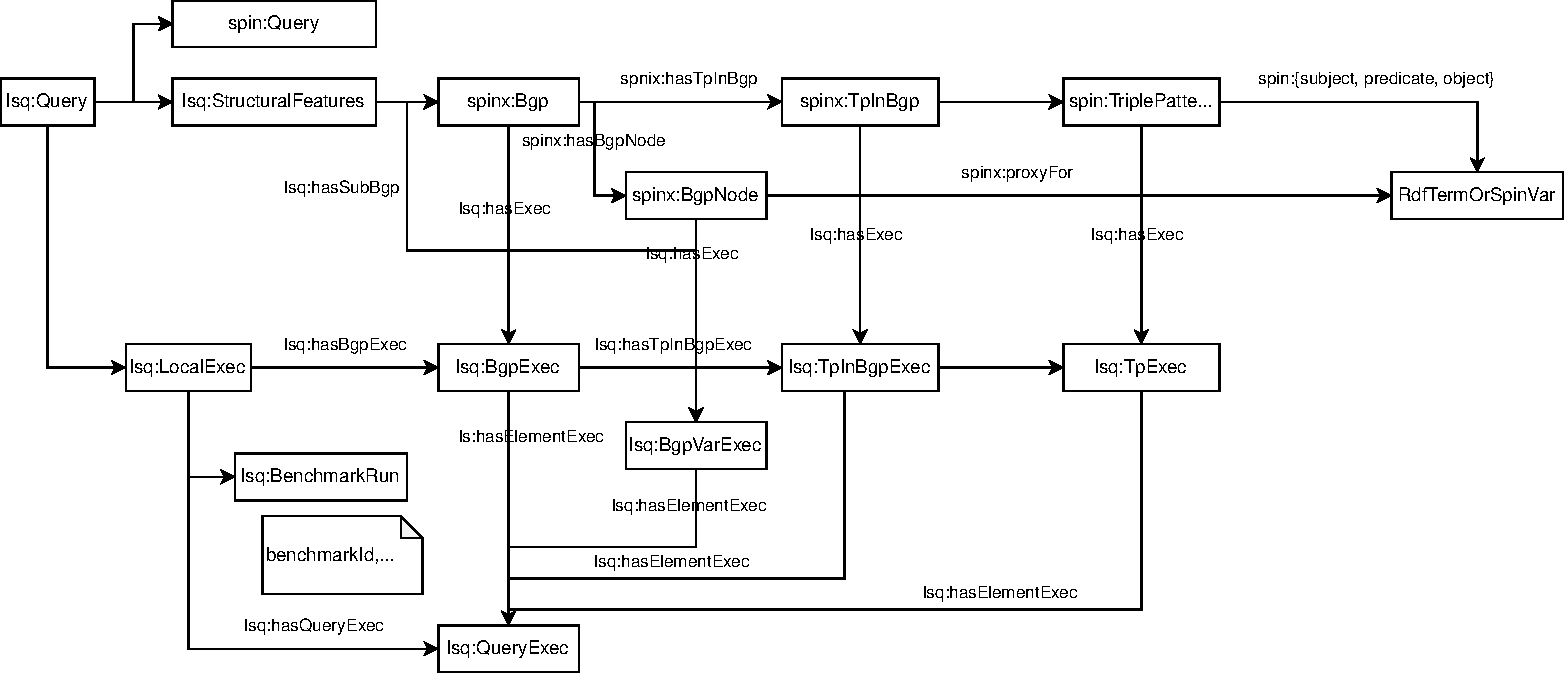
\includegraphics[width=\linewidth]{img/lsq2-datamodel}
%\caption{An overview of the LSQ data model, showing how different classes connect through different (object) properties}
%\label{fig:data_model}
%\end{figure*}

%\begin{comment}
\begin{figure*}
\centering
\begin{tikzpicture}[scale=0.73, every node/.style={transform shape}]

\tikzset{
	iri/.style={
		draw=black!50!white, 
		rectangle,
           	rounded corners,
           	thick,
           	text centered,
		top color=white, 
		bottom color=black!15, 
		font=\tt\small\hsp,
		inner sep=5pt,
		outer sep=0pt},
	lit/.style={
		draw=black!50!white, 
		rectangle,
		thick,
		text centered,
		top color=white, 
		bottom color=black!15, 
		font=\tt\small\hsp},
	arrout/.style={
		->,
		-latex,
		font=\tt\footnotesize\hsp},
	arrin/.style={
           	<-,
           	latex-,
		font=\tt\footnotesize\hsp}
}

\node[iri,anchor=center] (q) {
	\begin{tabular}{@{}l@{}}
	\multicolumn{1}{c}{lsqv:Query} \\
	\fbox{
	{\scriptsize
	\begin{tabular}{@{}l@{~~}l@{}}
	 lsqv:hash & (xsd:string)\\
	 lsqv:text & (xsd:string) \\
 	 lsqv:parseError & (xsd:string)
	\end{tabular}
	}
	}
	\end{tabular}
    };

\node[iri,anchor=center,below=3cm of q.center] (le) {lsqv:LocalExec}
 edge[arrin] node[fill=white,xshift=-0.4cm,pos=0.3] {lsqv:hasLocalExec} (q);
 
\node[iri,left=2.3cm of le.north west,anchor=north east] (re) {	
	\begin{tabular}{@{}l@{}}
	\multicolumn{1}{@{}c@{}}{lsqv:RemoteExec} \\
	\fbox{
		{\scriptsize
			\begin{tabular}{@{}l@{~~}l@{}}
			prov:atTtime & (xsd:dateTimeStamp) \\
			lsqv:hostHash & (xsd:string)
			\end{tabular}
		}
	}
	\end{tabular}}
  edge[arrin] node[fill=white] {lsqv:hasRemoteExec} (q);
  
\node[iri,anchor=center,below=2cm of re.center,dotted] (end) {cogs:Endpoint}
	edge[arrin] node[fill=white] {lsqv:endpoint} (re);

\node[iri,right=2cm of le.north east,anchor=north west] (sf) {
	\begin{tabular}{@{}l@{}}
	\multicolumn{1}{@{}c@{}}{lsqv:StructuralFeatures} \\
	\fbox{
		{\scriptsize
			\begin{tabular}{@{}l@{~~}l@{}}
			lsqv:bpgCount & (xsd:integer) \\			
			lsqv:joinVertexCount & (xsd:integer) \\
			lsqv:joinVertexDegreeMean & (xsd:decimal) \\
			lsqv:joinVertexDegreeMedian & (xsd:integer) \\
			lsqv:projectVarCount & (xsd:integer) \\
			lsqv:tpCount & (xsd:integer) \\
			lsqv:tpInBgpCountMax & (xsd:integer) \\
			lsqv:tpInBgpCountMean & (xsd:integer) \\			
			lsqv:tpInBgpCountMedian & (xsd:integer) \\			
			lsqv:tpInBgpCountMin & (xsd:integer) \\
			\end{tabular}
		}
	}
	\end{tabular}
	}
    edge[arrin] node[fill=white] {lsqv:hasStructuralFeatures} (q);
    
\node[iri,anchor=center,below=2cm of sf,dotted,xshift=4cm] (f) {sd:Feature}
	edge[arrin] node[fill=white] {lsqv:usesFeature} (sf);

\node[iri,anchor=center,below=2cm of sf] (bgp) {lsqv:Bgp}
	edge[arrin] node[fill=white] {lsqv:hasBgp} (sf);
	
\node[iri,anchor=center,left=2.4cm of bgp] (bgpe) {lsqv:BgpExec}
	edge[arrin] node[fill=white,pos=0.55] {lsqv:hasExec} (bgp);
	
%\node[iri,anchor=center,below=2cm of bgp] (ver) {...}
%	edge[arrin] node[fill=white] {lsqv:hasBgpNode} (bgp);

\node[iri,right=1cm of sf.north east,anchor=north west] (sq) {sp:Query}
 edge[arrin] node[fill=white,pos=0.6] {lsqv:hasSpin} (q);

\node[iri,anchor=center,below=1.3cm of sq.center,dotted] (t) {\begin{tabular}{@{}c@{}}sp:Select\\sp:Ask\\sp:Describe\\sp:Construct\end{tabular}}
  edge[arrout,dashed] node[auto] {} (sq);
  
\node[iri,anchor=center,below=3.75cm of le.center,xshift=-6cm] (e) {
	\begin{tabular}{@{}l@{}}
	\multicolumn{1}{@{}c@{}}{lsqv:QueryExec} \\
	\fbox{
		{\scriptsize
			\begin{tabular}{@{}l@{~~}l@{}}
			lsqv:countingDuration & (xsd:decimal) \\
			lsqv:evalDuration & (xsd:decimal) \\
			lsqv:resultCount & (xsd:integer) \\
			lsqv:serializedResult & (xsd:string) \\			
			prov:atTtime & (xsd:dateTimeStamp)
			\end{tabular}
		}
	}
	\end{tabular}
	}
    edge[arrin] node[fill=white,pos=0.4] {lsqv:hasQueryExec} (le)
    edge[arrin] node[fill=white,pos=0.55,inner sep=2pt] {lsqv:hasElementExec} (bgpe);

\node[iri,anchor=center,xshift=1.4cm] (act) at (le|-end) {
	lsqv:BenchmarkRun}
   edge[arrin] node[fill=white] {lsqv:benchmarkRun} (le);   
    
%\node[iri,anchor=center,left=4cm of sf] (bgp) { lsqv:Bgp }
%  edge[arrin] node[fill=white] {lsqv:hasBgp} (sf);
%
%\node[iri,anchor=center,above=4cm of bgp,xshift=-2cm] (ver) { lsqv:Edge }
%  edge[arrin] node[fill=white] {lsqv:hasBgpNode} (bgp);
%
%\node[iri,anchor=center,above=4cm of bgp,xshift=2cm] (tp) { lsqv:Tp }
%  edge[arrin] node[fill=white] {lsqv:hasTp} (bgp);
  
%\node[iri,anchor=center,below=1.5cm of jv.center] (t) {\begin{tabular}{@{}c@{}}lsqv:Star\\lsqv:Path\\lsqv:Hybrid\\lsqv:Sink\end{tabular}}
%edge[arrout,dashed] node[auto] {} (jv);     
    

  
\node[font=\scriptsize\tt,dashed,draw,anchor=north east] (pre) at (sq.east|-q.north)
{\begin{tabular}{@{$\!$}l@{~}l@{$\!$}} %
dct: & http://purl.org/dc/terms/\\
lsqv: & http://lsq.aksw.org/vocab\#\\ %
prov: & http://www.w3.org/ns/prov\#\\
sd: & http://www.w3.org/ns/sparql-service-description\#\\ %
sp: & http://spinrdf.org/sp\# %
\end{tabular}};
\end{tikzpicture}

%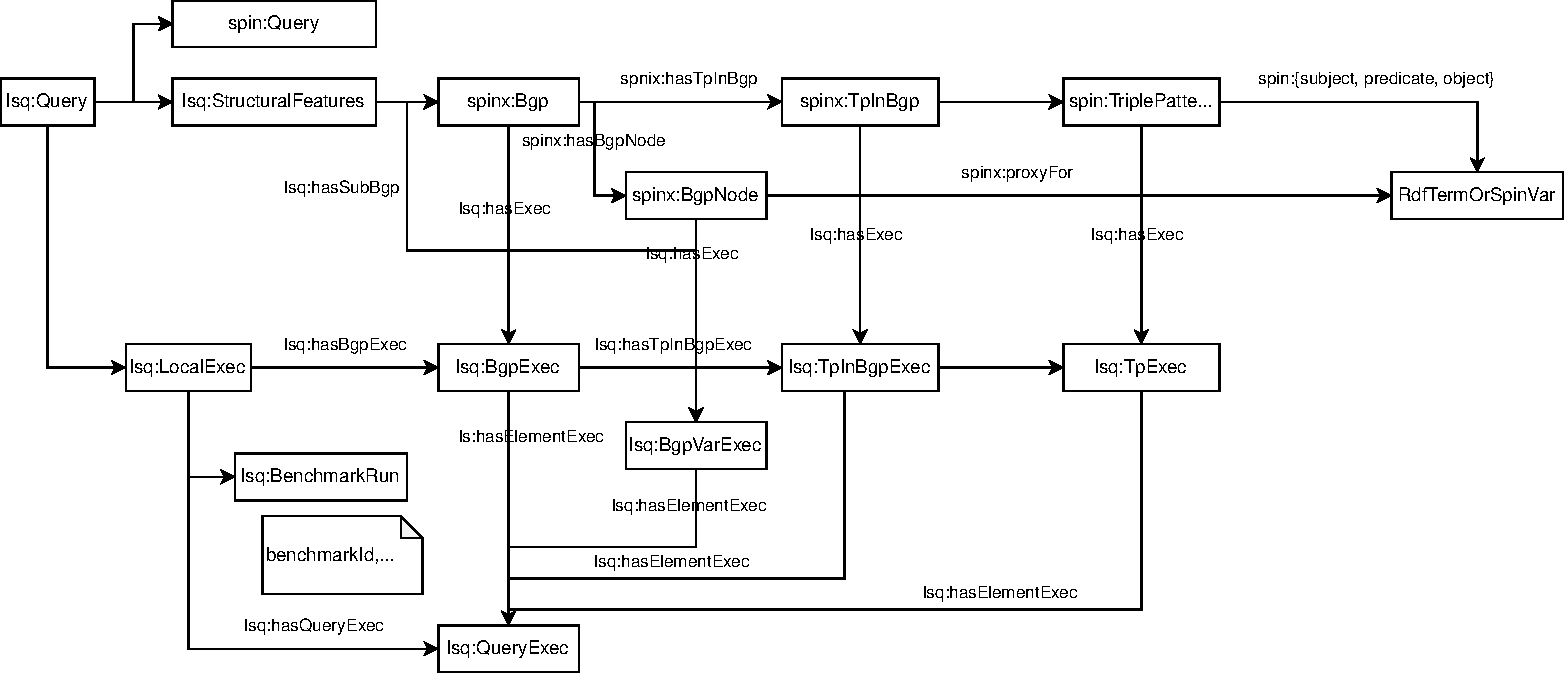
\includegraphics[width=\linewidth]{img/lsq2-datamodel}
\caption{Core of the LSQ data model: dashed lines indicate sub-classes; datatype properties are embedded within their associated class nodes to simplify presentation; external classes are shown with dotted borders. For clarity, we do not show details of the SPIN representation, or the execution of query elements more fine-grained than BGPs (which follow a similar pattern)}
\label{fig:data_model}
\end{figure*}
%\end{comment}

\begin{lstlisting}[caption = {An example LSQ/RDF representation of a SPARQL query in Turtle syntax},label = {lst:reprsentation},style=lst,basicstyle={\scriptsize\ttfamily},language=ttl,frame={single},breaklines=true,stepnumber=0,float=*]
@prefix rdf:	<http://www.w3.org/1999/02/22-rdf-syntax-ns#> .
@prefix lsqr:	<http://lsq.aksw.org/> .
@prefix lsqv:	<http://lsq.aksw.org/vocab#> .
@prefix rdfs:	<http://www.w3.org/2000/01/rdf-schema#> .
@prefix swc:	<http://data.semanticweb.org/ns/swc/ontology#> .
@prefix swr:	<http://data.semanticweb.org/> .
@prefix xsd:	<http://www.w3.org/2001/XMLSchema#> .
@prefix prov:	<http://www.w3.org/ns/prov#> .

# Primary resource describing the query found with the SWDF logs
lsqr:lsqQuery-3wBd2uKotB_-vUxnngs6ZNsGPhJmIDD9c7ig0UI24y8	
	lsqv:hasLocalExec lsqr:localExec-v9fBp3ElS1aVXXN1Z8zX1jxcHX3iy-axTgRrU2c7NY8 ;
	lsqv:hasRemoteExec lsqr:re-data.semanticweb.org-sparql_2014-05-22T16:08:17Z ,
		lsqr:re-data.semanticweb.org-sparql_2014-05-20T13:24:13Z ;
	lsqv:hasStructuralFeatures lsqr:lsqQuery-3wBd2uKotB_-vUxnngs6ZNsGPhJmIDD9c7ig0UI24y8-sf ;
	lsqv:hash "3wBd2uKotB_-vUxnngs6ZNsGPhJmIDD9c7ig0UI24y8" ;
	lsqv:text """PREFIX  rdf:  <http://www.w3.org/1999/02/22-rdf-syntax-ns#>
	               PREFIX  swc:  <http://data.semanticweb.org/ns/swc/ontology#>
	               SELECT DISTINCT  ?prop
	               WHERE { ?obj  rdf:type swc:SessionEvent ; ?prop ?targetObj FILTER isLiteral(?targetObj)  }
	               LIMIT   150""" .

# Static features of the query
lsqr:lsqQuery-3wBd2uKotB_-vUxnngs6ZNsGPhJmIDD9c7ig0UI24y8-sf	
	lsqv:bgpCount 1 ;
	lsqv:hasBgp lsqr:bgp-_x9Mckke-V9R3ddISuw-Nj_j278nT5HwiA1WUNk7tgY ;
	lsqv:joinVertexCount 1 ;
	lsqv:joinVertexDegreeMean 2 ;
	lsqv:joinVertexDegreeMedian 2 ;
	lsqv:projectVarCount 1 ;
	lsqv:tpCount 2 ;
	lsqv:tpInBgpCountMax 2 ;
	lsqv:tpInBgpCountMean 2 ;
	lsqv:tpInBgpCountMedian 2 ;
	lsqv:tpInBgpCountMin 2 ;
	lsqv:usesFeature lsqv:fn-isLiteral , lsqv:Select , lsqv:Limit , lsqv:Functions , lsqv:Group , lsqv:Filter , 
		lsqv:Distinct , lsqv:TriplePattern .              

# Remote execution no. 1 on the original endpoint
lsqr:re-data.semanticweb.org-sparql_2014-05-22T16:08:17Z	
	prov:atTime "2014-05-22T16:08:17Z"^^xsd:dateTime ;
	lsqv:endpoint swr:sparql ;
	lsqv:hostHash "O5UQpDtofxAsrJk7yzGfDolFGylMFw5446KcRZDcBkU" .

# Remote execution no. 2 on the original endpoint
lsqr:re-data.semanticweb.org-sparql_2014-05-20T13:24:13Z	
	prov:atTime "2014-05-20T13:24:13Z"^^xsd:dateTime ;
	lsqv:endpoint swr:sparql ;
	lsqv:hostHash "7aPNvqsgizRuEjH7_cO_dXoqLk-exKJ-xFmbCH3ew_E" .

# Local execution to extract statistics
lsqr:localExec-v9fBp3ElS1aVXXN1Z8zX1jxcHX3iy-axTgRrU2c7NY8-xc	
	lsqv:benchmarkRun lsqr:xc-swdf_2020-09-23_at_23-09-2020_17:10:19 ;
	lsqv:hasQueryExec lsqr:queryExec-Cmv7SccybbBxwkep_cHvDiF3piq29tH7NWlDfIiCHqU .

# Results of local execution
lsqr:queryExec-Cmv7SccybbBxwkep_cHvDiF3piq29tH7NWlDfIiCHqU	
	prov:atTime "2020-09-23T15:27:36.325Z"^^xsd:dateTime ;
	lsqv:countingDuration 0.008466651 ;
	lsqv:evalDuration 0.008868635 ;
	lsqv:resultCount 16 .
		
# The full data further include a SPIN description of the query, a list of BGPs within the query,
# a list of triple patterns and terms within the query, as well as execution statistics for individal
# BGPs, triple patterns and sub-BGPs induced by join variables
\end{lstlisting}

In Figure~\ref{fig:data_model} we provide an overview of the model used to represent queries in RDF, while in Listing~\ref{lst:reprsentation} we provide a snippet of the top-level data generated for a query found in the \swdf logs.\footnote{Note that for the purposes of presentation, we abbreviate some of the details of the query, including the IRIs used to identify local query executions.} We now discuss the groups of features described for each query.

\paragraph{Query instance} We define a ``query'' to be uniquely identified by the syntactic query string (independently of the endpoint, the particular execution, etc.). We type these queries with \texttt{lsqv:Query}. Instances of this class are linked to the query string using \texttt{lsqv:text}, and to various instances of local and remote executions. Other links are provided to other resources that capture further details of the static features of the query, its structure, as well as runtime statistics of its local execution (on our server) as information about its remote execution (on the original server).

\paragraph{Static features} Next we define some static features of the query, independent of the dataset over which it is evaluated. These include links to its individual join variables, triple patterns, and basic graph patterns; the SPARQL features that is uses; its number of projected variables, basic graph patterns, join variables, triple patterns; the maximum, mean and median degree of its join variables; and the maximum and minimum size of its basic graph patterns. The triple patterns and basic graph patterns themselves link to the SPIN representation of the query included in the description (and discussed presently); the triple patterns, in turn, link to the resources used by the query. The join variables, on the other hand, are described separately, indicating the degree of the variable and type of join~\cite{SaleemN14} it induces.

\paragraph{SPIN representation} While the static features aim to capture some high-level descriptions of the query that may be of interest to specific use cases, some details may be missing. In the interest of generality, we also include for each query a SPARQL Inferencing Notation (SPIN)~\cite{spin} representation of the query, which essentially captures a fine-grained translation of the SPARQL query to RDF. This SPIN encoding can be translated back to a SPARQL query equivalent to the original.\footnote{Given a query $Q$ and dataset $D$, let $Q(D)$ denote the result(s) of evaluating $Q$ over $D$. Two queries $Q_1$ and $Q_2$ are then defined to be \textit{equivalent} if and only if $Q_1(D) = Q_2(D)$ for every dataset $D$.} 

%Note that while Listing~\ref{lst:reprsentation} provides an example of the SPIN notation, for clarity, the model shown in Figure~\ref{fig:Schema} excludes most of the SPIN vocabulary, including onle some of the high-level sub-classes that indicate \texttt{SELECT}, \texttt{CONSTRUCT}, \texttt{ASK} and \texttt{DESCRIBE} queries.

\paragraph{Remote execution(s)} Next, individual queries are associated with one or more executions on the original endpoint, including a timestamp of when the query was executed, as well as an anonymised ID for the client---based on their cryptographically-hashed and salted I.P.---to identify which queries are run by the same agent.\footnote{A ``salt'' in cryptography is a privately-held arbitrary string that is combined (e.g., concatenated) with the input being hashed in order to avoid attacks based on precomputed tables (e.g., of common values or, in this case, of a collection of I.P.'s of interest).} The remote execution is also linked to the originating endpoint using \texttt{lsqv:endpoint}.\footnote{Although there exist properties called ``endpoint''---such as \texttt{void:sparqlEndpoint} or \texttt{sd:endpoint}---the domains of these properties were not query executions, but rather VoID datasets (i.e., sets of RDF triples), or SPARQL services. Though it would be possible to define properties such as \texttt{lsqv:dataset} or \texttt{lsqv:service} and then link a query execution \texttt{<x>} to an endpoint URL \texttt{<e>} with \texttt{<x> lsqv:dataset [ void:sparqlEndpoint <e> ]}, or alternatively \texttt{<x> lsqv:service [ sd:endpoint <e> ]}, this would introduce $O(n)$ additional triples to the LSQ~2.0 dataset, for $n$ the number of remote query executions (in LSQ~2.0, $n = 43,952,379$). (Please note that the dataset or service may change during the lifetime of the log, which we do not have information about; hence we cannot refer to one dataset/service at a given endpoint.) Thus we rather introduce \texttt{lsqv:endpoint} in the data and define property chain axioms in the LSQ~2.0 vocabulary to relate \texttt{lsqv:endpoint} to \texttt{lsqv:dataset}/\texttt{void:sparqlEndpoint} and \texttt{lsqv:service}/\texttt{sd:endpoint}.} Given that these meta-data constitute provenance for the query, we use the PROV Ontology (PROV-O)~\cite{prov-o} for modelling the time, date and agent involved in the remote execution.

\paragraph{Local execution} In most cases, the log of the remote executions will not provide statistics about the execution of the query in terms of how many results were returned, how long it took, how selective were the individual patterns, and so forth. Hence we re-execute the queries offline against the original dataset to generate runtime statistics about the query. Local executions were run on a machine with 64 core Intel(R) Xeon(R) CPU E5-2683 v4 @ 2.10GHz, and 528 GB RAM running Ubuntu 18.04.5 LTS using Virtuoso 7.2.\footnote{The configuration used for Virtuoso was \texttt{MaxQueryMem = 32G}, \texttt{NumberOfBuffers = 20050000}, and \texttt{MaxDirtyBuffers = 20000000}.} Due to the large number of queries to evaluate, we set a query timeout of one minute. The statistics generated include the number of results and the runtime for the query, as well as the number of results and the selectivity for each individual triple pattern.\footnote{The selectivity of the triple pattern is the ratio of triples from the dataset that it selects.} Runtime statistics are computed in a controlled environment that abstract away external factors such as the load on the endpoint server, etc.; however, due to the costs involved in evaluating such queries, we compute these only for one query engine, namely Virtuoso~7.2, where runtime estimates may thus vary for other engines.

\paragraph{Summary} The meta-data described in this section aim to strike a balance in terms of the four desiderata mentioned previously. In terms of \textbf{Generality}, we provide detailed meta-data for static query features, for provenance, and for runtime query statistics. In terms of \textbf{Conciseness}, though the detailed meta-data do require potentially many triples to be encoded for each query, we take steps to reduce this number by re-using resources insofar as appropriate where, for example, each unique query string is encoded once per log, with one set of static features, one SPIN representation, and one set of local executions, being subsequently linked to its different remote executions (rather than duplicate the former meta-data each time the same query string appears in the log). In terms of \textbf{Usability}, we provide some ``shortcut triples'' that allow for quickly finding queries of interest; for example, the static features of the query are largely of this form, where all such meta-data could in principle be computed from the SPIN representation, but using rather complex SPARQL queries over LSQ; the static query features are thus presented to make it easier to find queries, for example, with a certain range of numbers of triple patterns, or queries using \texttt{DISTINCT} and \texttt{GROUP BY}, etc. We will discuss \textbf{Linked Data Compatibility} in the section that follows.

\section{Publication}\label{sec:publish}

The LSQ dataset is published as Linked Data. Before describing the current contents of LSQ, we discuss in more detail how LSQ has been published.

\paragraph{Access Methods} We provide a number of ways to access LSQ. Firstly, following Linked Data principles, all IRIs under the \texttt{lsqr:} namespace are made dereferenceable using a \texttt{303 Redirect}; this is implemented with LodView\footnote{https://github.com/LodLive/LodView} and supports content negotiation. A SPARQL endpoint is provided for querying LSQ~2.0. Table~\ref{tab:access} lists the locations for these access methods.

\begin{table*}
\centering
\setlength\columnsep{10pt}
\setlength{\tabcolsep}{3ex}
\caption{Locations from which LSQ can be accessed including an example Linked Data IRI, the vocabulary, dumps, the SPARQL endpoint, as well as locations where LSQ is indexed, including DataHub, Linked Open Vocabularies (LOV) and prefix.cc}
\label{tab:access}
\begin{tabular}{l@{~~~}l}
\toprule
\textbf{Method} & \textbf{Location}\\
\midrule
Linked Data IRIs & \url{http://lsq.aksw.org/lsqQuery-3wBd2uKotB_-vUxnngs6ZNsGPhJmIDD9c7ig0UI24y8} (\textit{example}) \\
Vocabulary & \url{http://lsq.aksw.org/vocab} \\
Dumps       	 & \url{http://lsq.aksw.org/downloads} \\
SPARQL Endpoint  & \url{http://lsq.aksw.org/sparql} \\
\midrule
\textbf{Catalogue} & \textbf{Location}\\
\midrule
Datahub		& \url{https://datahub.io/dataset/lsq} \\
LOV			& \url{https://lov.linkeddata.es/dataset/lov/vocabs/lsq} \\
prefix.cc	& \url{http://prefix.cc/lsqv} \\
\bottomrule
\end{tabular}
\end{table*}

\paragraph{Vocabulary} As seen in Figure~\ref{fig:data_model}, we use a mixture of a custom vocabulary in the \texttt{lsqv:} namespace, as well as existing vocabulary where possible. The custom LSQ vocabulary dereferences (via \texttt{303 Redirect}) to an RDFS/OWL definition of the corresponding terms in Turtle, which includes metadata about authors. The vocabulary meets four of the five stars of Linked Data vocabulary use~\cite{JanowiczHAKV14}.\footnote{With respect to the fifth star, which requires that our LSQ vocabulary be \textit{linked to} from external vocabularies, we are not aware of such links, though we do know, for example, that Varga et al.~\cite{varga2018analytical} incorporate elements of the LSQ vocabulary within their own Analytical Metadata (AM) model, while Singh et al.~\cite{singh2019qaldgen} also use the LSQ vocabulary within their benchmark.} With respect to external vocabulary, we re-use terms from the SPARQL Inferencing Notation (SPIN) ontology~\cite{spin}, as well as the Provenance Ontology (PROV-O)~\cite{prov-o} where possible.%\footnote{We have avoided re-using inappropriate terms. For example, we use \texttt{lsqv:endpoint} rather than \texttt{void:sparqlEndpoint} or \texttt{sd:endpoint} as the former has a query execution as its domain, while the latter have a dataset and a service as their domain, respectively.}

\paragraph{Discoverability} The LSQ dataset has been registered in the DataHub catalogue, while the LSQ vocabulary has been listed on Linked Open Vocabularies (LOV)~\cite{VandenbusscheAP17} as well as prefix.cc. We provide these locations in Table~\ref{tab:access}. We also compute and publish meta-data about the LSQ dataset using the Vocabulary of Interlinked Datasets (VoID)~\cite{key:void}. More specifically, we compute a separate VoID description for each log and make the resulting description accessible via both a downloadable file and a named graph of the SPARQL endpoint.

\paragraph{Availability} The LSQ dataset has been hosted for over six years (at the time of writing) by the Agile Knowledge Engineering and Semantic Web (AKSW) group. As discussed in Section~\ref{sec:lsq_adoption}, it has been widely adopted in that time. The dataset is available to all under a CC-BY license. We further make the source code used for generating the LSQ dataset from the raw query logs available on Github \url{https://github.com/AKSW/LSQ}.

\section{LSQ~2.0 Logs}\label{sec:logs}

We now describe the content of the LSQ~2.0 dataset. In order to collect raw SPARQL query logs, we sent mails both to the \texttt{public-lod@w3.org} mailing list and to individual providers of endpoints. We also incorporated logs from LSQ~1.0~\cite{SaleemAHMN15} and a sample of queries from the Wikidata logs~\cite{MalyshevKGGB18}. We thus acquired access to the logs of 27 endpoints, 22 of which are part of Bio2RDF release 3~\cite{DumontierCCAEBD14}.\footnote{We also acquired logs for the British Museum and UniProt endpoints, but decided to omit them due to having few unique queries.} Table~\ref{tab:dsbstats} provides high-level statistics of the query logs from which we extract the LSQ dataset, including the query executions registered; the unique query strings; the number of queries providing a runtime error, or returning zero results; as well as the percentage of unique queries using \texttt{SELECT}, \texttt{CONSTRUCT}, \texttt{DESCRIBE} or \texttt{ASK}. Aside from the initial log of LSQ, only one log is already publicly available, namely Wikidata~\cite{MalyshevKGGB18}, of which we include a subset described in our data model.


% In Table~\ref{tab:lsqstats}, we provide statistics of the dataset over which the queries were executed, including the unique subjects, predicates, objects and triples per dataset, as well as the location of the SPARQL endpoint. 
  
\paragraph{\affymetrix} is a biomedical Linked Dataset describing probesets found in DNA microarrays~\cite{DumontierCCAEBD14}.

\paragraph{\biomodels} is a biomedical Linked Dataset describing mathematical models of biological systems~\cite{DumontierCCAEBD14}.\footnote{The external SPARQL endpoint is spelt \texttt{biomedels}, and thus the IRIs use this spelling in LSQ~2.0.}

\paragraph{BioPortal} is a biomedical Linked Dataset cataloguing biomedical ontologies~\cite{DumontierCCAEBD14}.

\paragraph{\ctd: Comparative Toxicogenomics Database} is a biomedical Linked Dataset that describes how environmental chemicals relate to diseases~\cite{DumontierCCAEBD14}.

\paragraph{\dbpedia} is a cross-domain Linked Dataset that is primarily extracted from Wikipedia~\cite{LehmannIJJKMHMK15}.

\paragraph{\dbsnp: Single Nucleotide Polymorphism Database} is a biomedical Linked Dataset that describes single base nucleotide substitutions and short deletion and insertion polymorphisms~\cite{DumontierCCAEBD14}.

\paragraph{\drugbank} is a biomedical Linked Dataset that describes drugs and drug targets~\cite{DumontierCCAEBD14}.

\paragraph{\genage} is a biomedical Linked Dataset that describes human and other genes linked with ageing~\cite{DumontierCCAEBD14}.

\paragraph{\gendr: Dietary Restriction Gene Database} is a biomedical Linked Dataset that describes genes associated with dietary restrictions~\cite{DumontierCCAEBD14}.

\paragraph{\go: Gene Ontology} is a biomedical ontology that describes gene, gene products, and their functions~\cite{DumontierCCAEBD14}.

\paragraph{\goa: Gene Ontology Annotation} is a biomedical Linked Dataset that provides annotations on proteins, RNA and protein complexes~\cite{DumontierCCAEBD14}.

\paragraph{\hgnc: HUGO Gene Nomenclature Committee} is a biomedical Linked Dataset that describes human gene nomenclature~\cite{DumontierCCAEBD14}.

\paragraph{\irefindex} is a biomedical Linked Dataset that indexes interaction data for proteins~\cite{DumontierCCAEBD14}.

\paragraph{\kegg: Kyoto Encyclopedia of Genes and Genomes} is a biomedical Linked Dataset that describes functions of genes and biological systems~\cite{DumontierCCAEBD14}.

\paragraph{\linkedgeodata} is a geographical Linked Data extracted primarily from Open Street Map~\cite{StadlerLHA12}.

\paragraph{\linkedspl: Linked Structured Product Labelling} is a biomedical Linked Dataset that contains meta-data about drug labels sourced from DailyMed~\cite{DumontierCCAEBD14}.

%\paragraph{Life Science Resource Registry (LSR)} is a biomedical Linked Dataset that contains terminological resources relating to the life sciences~\cite{DumontierCCAEBD14}. \ah{No longer in Table 2} \ah{Not in the endpoint.}

%\paragraph{Medical Subject Headings (MeSH)} is a biomedical Linked Dataset that describes a taxonomy for cataloguing biomedical information~\cite{DumontierCCAEBD14}. \ah{No longer in Table 2} \ah{Not in the endpoint.}

\paragraph{\mgi: Mouse Genome Informatics} is a biomedical Linked Dataset that describes mouse genes, alleles, and strains~\cite{DumontierCCAEBD14}.

\paragraph{NCBI Gene} is a biomedical Linked Dataset that describes gene-related information given by the National Center for Biotechnology Information (NCBI)~\cite{DumontierCCAEBD14}.

%\paragraph{National Drug Code (NDC)} is a biomedical Linked Dataset that describes unique product identifiers for drugs intended for human consumption in the United States~\cite{DumontierCCAEBD14}. %\ah{stats} 
%\ah{No longer in Table 2.} \ah{Not in the endpoint.}

\paragraph{Online Mendelian Inheritance in Man (\omim)} is a biomedical Linked Dataset that catalogues human genes as well as genetic traits and disorders~\cite{DumontierCCAEBD14}. %\ah{stats}

%\paragraph{Orphanet} is a biomedical Linked Dataset that describes rare diseases and orphan drugs~\cite{DumontierCCAEBD14}. \ah{No longer in Table 2.} \ah{Not in the endpoint.} 

\paragraph{\pharmgkb} is a biomedical Linked Dataset describing how genetic variations impact drug responses~\cite{DumontierCCAEBD14}. %\ah{stats}

\paragraph{\sabiork: System for the Analysis of Biochemical Pathways -- Reaction Kinetics} is a biomedical Linked Dataset that describes biochemical reactions~\cite{DumontierCCAEBD14}. %\ah{stats}

\paragraph{\sgd: Saccharomyces Genome Database} is a biomedical Linked Dataset describing the biology and genetics of the yeast \textit{Saccharomyces cerevisiae}~\cite{DumontierCCAEBD14}. %\ah{stats}

\paragraph{\sider: Side Effect Resource} is a biomedical Linked Dataset describing the side effects of drugs~\cite{DumontierCCAEBD14}. %\ah{stats}

\paragraph{\swdf: Semantic Web Dog Food} is a bibliographical Linked Dataset describing papers, presentations and people participating in top Semantic Web related conferences and workshops~\cite{MollerHHD07}. 

\paragraph{\taxonomy: NBCI Taxonomy} is a biomedical Linked Dataset that describes all organisms found in genetic databases~\cite{DumontierCCAEBD14}.

\paragraph{\wikidata} is a collaboratively edited knowledge graph hosted by the Wikimedia foundation~\cite{MalyshevKGGB18}. 

\paragraph{\wormbase} is a biomedical Linked Dataset that describes the biology and genome of worms~\cite{DumontierCCAEBD14}. 

%\ah{data stats} The Semantic Web Dog Food (\swdf) log spans from May 16, 2014 to November 12, 2014 and records over 1.4 million query executions.

%\paragraph{UniProt} \ah{include?}


%\subsubsection{British Museum} provides a Linked Data representation of an online collection containing records of more than 3 million artefacts. The British Museum (BM) Linked Dataset is accessible at \url{http://collection.britishmuseum.org/sparql} through an OWLIM/GraphDB interface. The log we have acquired spans from November 8, 2014 to December 1, 2014 and contains over 800 thousand query executions.

%\subsubsection{Overview of datasets}
%In Table~\ref{tab:dsbstats}, we present some high-level statistics of the \textit{original} Linked Datasets corresponding to the time of the logs (e.g., \dbpedia refers to \dbpedia v.3.5.1), including the number of distinct triples, subjects, predicates, objects and classes over which queries would have been issued. The statistics were collected by downloading and locally analysing the data. These datasets will be used later to generate controlled estimates of data-sensitive statistics for queries, such as runtimes, result sizes, triple pattern selectivity, etc.


%\newcommand{\cenh}[1]{\multicolumn{1}{c}{#1}}




\section{LSQ~2.0 Query Statistics}\label{sec:queries}

We now look in more detail at the composition of the queries currently included in the LSQ dataset. In particular, we first look at some high-level statistics for queries in the dataset, before looking at the static features of the query, the agents making the queries, as well as runtime statistics computed against the corresponding dataset. Finally we discuss the composition of the LSQ dataset itself.

%We applied the RDFisation process to the four logs mentioned in the previous section. Given that the logs were in different formats, we created custom scripts to extract and normalise data from the four different sources, mapping them to the target schema outlined in Section~\ref{sec:model}. We now give a more in-depth analysis of the resulting datasets, as well as an analysis of the unique queries, query executions and agents mentioned therein. Our goal is to provide insights into the scope and usefulness of the dataset, as well as its limitations.




%Bullets for Aidan from Mario report
%\begin{itemize}
%\item 2 datasets DBLP and \swdf 5 million and 2 million queries respectively.
%\item Select most common used operator 96.9 in \dbpedia , ask 1.6 construct 1.5 and describe .002 , In \swdf select is 99.7
%\item Filter most common operator 49 percent both
%\item Lang most used function only in \dbpedia and obvious because of it support for multiple languages, second most used function is EQUAL (dblp 23 percent) and \swdf top most 93 percent.
%\item Distinct more popular on \dbpedia than \swdf
%\item lack of usage of features like Order BY, GRAPH, FROM , FROM NAMED and OFFSET
%\item UNION is 11.84 for \dbpedia while for OPTIONAL they said significant
%\item triple pattern number, 66 percent in \dbpedia and 97.25 in \swdf contain a single triple pattern
%\item 6 types of joins , SS, SO, SP, PP, PO, OO . SS is most used almost 60 $\%$ in both while SO is second most common around 35 while OO is almost 5, rest are negligible. 
%\end{itemize}

\paragraph{High-level statistics:} Table~\ref{tab:dsbstats} provides a high-level analysis of the queries (both query executions and unique queries) appearing in each of the logs considered. From the overall row, we see that LSQ contains 43.95 million query executions and 11.56 million unique queries, implying that each query is executed, on average, 3.8 times within each log. Of the unique queries, 7.7 million (66.9\%) have runtime errors; and 2.3 million (20.0\%) have no errors but return empty results. A high ratio of runtime errors come from the Bio2RDF logs. The majority of queries are \texttt{CONSTRUCT} queries (60.0\%), followed by \texttt{SELECT} (32.3\%), \texttt{DESCRIBE} (7.1\%) and \texttt{ASK} (0.5\%). We find that \texttt{CONSTRUCT} queries are particularly prevalent on Bio2RDF endpoints, while \texttt{DESCRIBE} queries are particularly prevalent on \dbpedia and Wikdata endpoints, possibly due to the use of such queries for dereferencing Linked Data IRIs through the endpoint.

\newcommand{\cenh}[1]{#1}

\begin{table*}
\setlength{\tabcolsep}{1.3ex}
\centering
\caption{High-level statistics for queries in the LSQ dataset (QE = Query Executions, UQ = Unique Queries, RE = Runtime Error, ZR = Zero Results, \texttt{SEL} = \texttt{SELECT}, \texttt{CON} = \texttt{CONSTRUCT}, \texttt{DES} = \texttt{DESCRIBE})}
\label{tab:dsbstats}
\begin{tabular}{lrrrrrrrr}
\toprule
\textsc{Dataset} & \cenh{\textsc{QE}} & \cenh{\textsc{UQ}} & \cenh{\textsc{RE}} & \cenh{\textsc{ZR}} & \cenh{\textsc{\texttt{SEL} (\%)}} & \cenh{\textsc{\texttt{CON} (\%)}} & \cenh{\textsc{\texttt{DES} (\%)}} & \cenh{\textsc{\texttt{ASK} (\%)}} \\
\midrule
\affymetrix	&	1,229,339	&	311,096	&	277,983	&	31,659	&	16.47	&	83.21	&	0.02	&	0.30	\\
\biomodels	&	1,238,375	&	435,232	&	412,984	&	21,692	&	41.18	&	58.75	&	0.00	&	0.06	\\
BIOPORTAL	&	1,337,804	&	89,664	&	85,273	&	3,389	&	64.88	&	34.78	&	0.00	&	0.34	\\
\ctd	&	940,390	&	287,296	&	266,999	&	19,824	&	11.98	&	87.76	&	0.00	&	0.26	\\
\dbpedia	&	6,535,500	&	4,258,941	&	1,259,972	&	1,755,338	&	69.90	&	3.59	&	25.23	&	1.28	\\
\dbsnp	&	794,023	&	269,498	&	267,662	&	1,698	&	4.99	&	94.99	&	0.00	&	0.02	\\
\drugbank	&	1,613,951	&	379,233	&	372,022	&	6,186	&	46.67	&	52.80	&	0.05	&	0.48	\\
\genage	&	589,211	&	265,067	&	263,205	&	1,661	&	5.55	&	94.43	&	0.00	&	0.02	\\
\gendr	&	690,864	&	270,697	&	262,776	&	7,726	&	7.53	&	92.45	&	0.00	&	0.02	\\
\go	&	1,839,991	&	121,542	&	88,743	&	30,082	&	98.31	&	0.03	&	0.35	&	1.31	\\
\goa	&	3,544,273	&	343,836	&	310,800	&	32,317	&	26.18	&	73.69	&	0.06	&	0.07	\\
\hgnc	&	1,529,681	&	364,961	&	327,540	&	33,568	&	29.15	&	70.58	&	0.04	&	0.23	\\
%HOMOLOGENE	&	1,242,694	&	321,061	&	1765	&	0	&	0.00	&	0.00	&	0.00	&	0.00	\\
\irefindex	&	1,560,704	&	309,777	&	289,546	&	19,858	&	18.10	&	81.88	&	0.00	&	0.02	\\
\kegg	&	66,830	&	19,871	&	10,386	&	8,004	&	92.04	&	4.30	&	0.41	&	3.24	\\
\linkedgeodata	&	154,884	&	61,897	&	11,028	&	13,990	&	98.58	&	1.00	&	0.02	&	0.40	\\
\linkedspl	&	337,001	&	204,112	&	203,534	&	310	&	0.28	&	99.69	&	0.00	&	0.03	\\
\mgi	&	1,316,673	&	319,627	&	277,080	&	33,781	&	21.12	&	78.60	&	0.05	&	0.23	\\
\ncbigene	&	770,716	&	216,832	&	215,938	&	718	&	8.71	&	91.26	&	0.00	&	0.04	\\
\omim	&	1,506,621	&	335,541	&	290,483	&	44,093	&	22.78	&	76.89	&	0.08	&	0.26	\\
\pharmgkb	&	94,540	&	24,000	&	14,597	&	8,649	&	60.35	&	39.65	&	0.00	&	0.01	\\
\sabiork	&	922,407	&	274,098	&	253,733	&	19,938	&	7.91	&	92.07	&	0.00	&	0.02	\\
\sgd	&	973,281	&	318,641	&	309,593	&	7,199	&	16.06	&	80.53	&	0.30	&	3.12	\\
\sider	&	599,285	&	277,766	&	274,963	&	1,965	&	9.38	&	90.59	&	0.00	&	0.03	\\
\swdf	&	1,415,567	&	101,423	&	30,792	&	36,789	&	73.57	&	0.06	&	26.17	&	0.21	\\
\taxonomy	&	7,698,898	&	354,582	&	334,290	&	20,041	&	15.83	&	84.16	&	0.00	&	0.02	\\
\wikidata	&	3,298,254	&	844,256	&	520,976	&	150,395	&	95.03	&	0.13	&	0.08	&	4.77	\\
\wormbase	&	1,353,316	&	498,170	&	496,325	&	1,660	&	49.33	&	50.66	&	0.00	&	0.01	\\
\midrule
Overall	&	43,952,379	&	11,557,656
		&	7,729,223	&	2,312,530	&	36.14	&	57.8	&	1.89	&	0.60	\\
\bottomrule
\end{tabular}
\end{table*}


\paragraph{Static features:} Turning to static features, we first look at the percentages of unique queries without parse errors using different SPARQL features (note that we will analyse joins in BGPs and property paths later). Table~\ref{tab:distfeatures} provides statistics for the usage of different features of SPARQL. We see that \texttt{FILTER} is among the most widely used features, along with SPARQL functions and expressions (note that almost all filters use such expressions). This feature is followed by \texttt{DISTINCT} and other solution modifiers, \texttt{UNION}, \texttt{OPTIONAL}, etc. Notably these are all SPARQL~1.0 features. The \texttt{SERVICE} keyword is commonly used on \wikidata since the Wikidata Query Service provides a custom service for retrieving multilingual labels as preferred/available.


\begin{table*}[!tb]
\setlength{\tabcolsep}{0.6ex}
\centering
\caption{Percentage of unique queries without parse errors using the specified SPARQL feature (\textsc{Sol. Mod.} includes the solution modifiers \texttt{ORDER BY}, \texttt{OFFSET}, and \texttt{LIMIT}; \textsc{Agg.} includes aggregation features \texttt{GROUP BY}, \texttt{HAVING}, \texttt{AVG}, \texttt{SUM}, \texttt{COUNT}, \texttt{MAX}, and \texttt{MIN}; \textsc{Neg.} includes \texttt{MINUS}, \texttt{NOT EXISTS}, and \texttt{EXISTS}; \textsc{Bind.} includes \texttt{VALUES} and \texttt{BINDING}; \textsc{Graph} includes \texttt{FROM}, \texttt{FROM NAMED}, and \texttt{GRAPH}; \textsc{Func.} includes SPARQL functions and expressions)} 
\label{tab:distfeatures}
\begin{tabular}{lrrrrrrrrrrrrr} \toprule
\textsc{Dataset} & \texttt{UNION} & \texttt{OPTIONAL} & \texttt{DISTINCT} & \texttt{FILTER} & \texttt{REGEX} & \texttt{SERVICE} & \textsc{Sub-Q.} & \textsc{Sol. M.} & \textsc{Agg.} & \textsc{Neg.} & \textsc{Bind.} & \textsc{Graph}  & \textsc{Func.} \\  \midrule
\affymetrix & 3.68 & 0.02 & 7.64 & 83.30 & 0.15 & 0.01 & 0.06 & 4.85 & 0.36 & 0.00 & 0.01 & 0.69 & 83.30 \\
\biomodels & 2.64 & 0.01 & 0.18 & 94.32 & 0.06 & 0.00 & 0.01 & 0.12 & 0.10 & 0.00 & 0.00 & 0.03 & 94.32 \\
BIOPORTAL & 1.50 & 0.06 & 0.05 & 37.95 & 2.23 & 0.01 & 0.01 & 0.21 & 34.10 & 0.00 & 0.00 & 34.26 & 37.95 \\
\ctd & 3.99 & 0.02 & 0.37 & 88.06 & 0.06 & 0.04 & 0.01 & 3.57 & 0.13 & 0.00 & 0.01 & 3.21 & 88.06 \\
\dbpedia & 28.68 & 19.97 & 22.22 & 29.87 & 4.10 & 0.00 & 2.22 & 8.92 & 9.98 & 0.00 & 1.11 & 0.01 & 29.87 \\
\dbsnp & 0.05 & 0.01 & 0.10 & 94.87 & 0.00 & 0.05 & 0.01 & 0.13 & 0.07 & 0.00 & 0.00 & 0.09 & 94.87 \\
\drugbank & 2.58 & 15.55 & 12.37 & 54.67 & 1.81 & 0.10 & 0.02 & 9.31 & 2.59 & 0.00 & 0.01 & 2.73 & 54.67 \\
\genage & 0.00 & 0.01 & 0.08 & 94.37 & 0.00 & 0.00 & 0.01 & 0.06 & 0.07 & 0.00 & 0.00 & 0.02 & 94.37 \\
\gendr & 0.01 & 0.01 & 0.07 & 96.55 & 0.00 & 0.01 & 0.01 & 0.06 & 0.07 & 0.00 & 0.00 & 0.02 & 96.55 \\
\go & 9.08 & 0.16 & 20.98 & 18.82 & 5.92 & 0.89 & 0.07 & 3.86 & 0.08 & 0.00 & 0.01 & 0.02 & 18.82 \\
\goa & 4.17 & 0.01 & 5.00 & 84.76 & 9.15 & 0.86 & 0.03 & 0.71 & 0.09 & 0.00 & 0.00 & 0.44 & 84.76 \\
\hgnc & 3.16 & 0.02 & 5.00 & 84.12 & 0.04 & 0.03 & 0.02 & 1.20 & 0.44 & 0.00 & 0.00 & 0.47 & 84.12 \\
\irefindex & 9.99 & 1.00 & 0.86 & 83.37 & 2.29 & 0.01 & 0.01 & 0.87 & 0.12 & 0.00 & 0.00 & 0.74 & 83.37 \\
\kegg & 11.64 & 1.13 & 54.91 & 7.22 & 2.86 & 0.07 & 0.04 & 42.95 & 1.02 & 0.00 & 0.01 & 0.79 & 7.22 \\
\linkedgeodata & 1.15 & 19.13 & 9.24 & 18.06 & 2.61 & 0.01 & 7.64 & 30.75 & 37.57 & 0.00 & 0.52 & 2.52 & 18.06 \\
\linkedspl & 0.00 & 0.01 & 0.00 & 99.76 & 0.00 & 0.00 & 0.01 & 0.05 & 0.07 & 0.00 & 0.00 & 0.03 & 99.76 \\
\mgi & 3.57 & 0.02 & 6.99 & 79.43 & 0.43 & 0.01 & 0.03 & 2.98 & 0.57 & 0.00 & 0.05 & 0.64 & 79.43 \\
\ncbigene & 0.02 & 0.01 & 0.17 & 91.53 & 0.02 & 0.03 & 0.01 & 2.72 & 0.22 & 0.00 & 0.00 & 2.61 & 91.53 \\
\omim & 3.52 & 1.10 & 4.90 & 80.83 & 0.31 & 0.39 & 0.04 & 5.62 & 0.93 & 0.00 & 0.01 & 1.09 & 80.83 \\
\pharmgkb & 33.05 & 0.00 & 42.22 & 47.92 & 0.28 & 0.13 & 0.01 & 43.40 & 0.07 & 0.00 & 0.00 & 1.14 & 47.92 \\
\sabiork & 4.15 & 0.01 & 0.12 & 92.00 & 0.00 & 0.00 & 0.01 & 0.17 & 0.09 & 0.00 & 0.00 & 0.05 & 92.00 \\
\sgd & 1.63 & 0.01 & 6.73 & 80.06 & 0.09 & 0.03 & 0.04 & 4.38 & 3.87 & 0.00 & 0.00 & 4.24 & 80.06 \\
\sider & 0.02 & 0.01 & 7.44 & 90.87 & 0.00 & 0.03 & 0.01 & 7.42 & 0.09 & 0.00 & 0.00 & 0.73 & 90.87 \\
\swdf & 40.13 & 34.08 & 53.16 & 2.34 & 0.87 & 0.04 & 0.10 & 31.45 & 1.08 & 0.00 & 0.01 & 32.32 & 2.34 \\
\taxonomy & 3.19 & 0.01 & 0.04 & 92.91 & 0.04 & 0.00 & 0.01 & 0.35 & 0.25 & 0.00 & 0.00 & 0.44 & 92.91 \\
\wikidata & 9.27 & 29.21 & 15.32 & 26.48 & 1.13 & 54.38 & 7.44 & 40.72 & 7.99 & 0.00 & 8.99 & 0.00 & 26.48 \\
\wormbase & 14.16 & 4.46 & 0.12 & 69.92 & 9.69 & 1.58 & 0.00 & 0.27 & 0.63 & 0.00 & 0.00 & 0.82 & 69.92 \\
\midrule
Overall & 7.22 & 4.67 & 10.23 & 67.57 & 1.63 & 2.17 & 0.66 & 9.14 & 3.77 & 0.00 & 0.34 & 3.34 & 67.57 \\
\bottomrule
\end{tabular}
\end{table*}

Next, in Table~\ref{tab:bgppp}, we provide three types of statistics about the basic graph patterns and property path features used. First, we present the unique number of subject, predicate and object terms used in the BGPs of the logs in order to characterise their diversity. We see that \dbpedia, \linkedgeodata and \wikidata offer the most diversity, particularly in terms of predicates found in the queries. Second, we present the percentage of queries with different types of joins in the basic graph patterns~\cite{SaleemN14}. Each join variable in a basic graph pattern is analysed in order to understand how they connect triple patterns. We say that a join vertex has an ``outgoing link'' if it appears as a subject of a triple pattern, and that it has an ``incoming link'' if it appears as predicate or object. The join types are then defined as follows:
\begin{description}
\item[{\textsc{Star}}] has multiple outgoing but no incoming links.
\item[{\textsc{Path}}] has one incoming and one outgoing link.
\item[{\textsc{Hybrid}}] has at least one incoming and outgoing link and three or more links overall.
\item[{\textsc{Sink}}] has multiple incoming but no outgoing links.
\end{description}
\noindent
From Table~\ref{tab:bgppp}, we see that the majority of queries have no joins, but where present, \textsc{Star} joins are the most frequent, followed by  \textsc{Hybrid} and \textsc{Sink} joins. Third, we present the number of queries using different property path features, where we see that \dbpedia and \wikidata contain the most use of property path queries, while Bio2RDF logs exhibit little use of this feature. The most used such feature is \texttt{/} for concatenation.

These statistics may be helpful for consumers to choose which dataset/log to work with. For example, for the purposes of benchmarking joins, a dataset such as \linkedgeodata or \wikidata may be chosen as most queries feature joins; in order to benchmark or analyse property paths, \dbpedia or \wikidata may be chosen as they use this feature more frequently; etc. 


\begin{table*}
\setlength{\tabcolsep}{1.1ex}
\centering
\caption{Analysis of basic graph patterns and property paths including number of unique subject/predicate/object terms, percentage of unique queries containing different types of joins (a query may contain multiple join types), and number of queries using different types of property path expressions (\texttt{/} denotes concatenation, \texttt{\textasciicircum} denotes inverse, \texttt{*} denotes zero-or-more; \texttt{+} denotes one-or-more; \cenh{\texttt{|}} denotes disjunction}
\begin{tabular}{lrrrrrrrrrrrrr} \toprule
\multirow{2}{*}{\textsc{Dataset}} & \multicolumn{3}{c}{\textsc{BGP Terms}} & \multicolumn{5}{c}{\textsc{Join Types (\%)}} & \multicolumn{5}{c}{\textsc{Prop. Path Features}} \\ 

& \cenh{\textsc{Subj.}} & \cenh{\textsc{Pred.}} & \cenh{\textsc{Obj.}} & \cenh{\textsc{Star}} & \cenh{\textsc{Hyb.}} & \cenh{\textsc{Path}} & \cenh{\textsc{Sink}} & \cenh{\textsc{None}} & \cenh{\texttt{/}} & \cenh{\texttt{\textasciicircum}} & \cenh{\texttt{*}} & \cenh{\texttt{+}} & \cenh{\texttt{|}} \\
\cmidrule(r){1-1}\cmidrule(lr){2-4}\cmidrule(lr){5-9}\cmidrule(l){10-14}
%\midrule
\affymetrix & 17,912 & 432 & 27,398 & 2.36 & 0.16 & 0.03 & 0.10 & 97.57 & 2 & 0 & 0 & 0 & 1 \\
\biomodels & 14,055 & 347 & 120,148 & 37.22 & 0.10 & 0.01 & 0.04 & 62.71 & 2 & 0 & 0 & 0 & 1 \\
BIOPORTAL & 9,275 & 130 & 6,275 & 36.26 & 34.22 & 0.01 & 53.08 & 44.60 & 1 & 0 & 0 & 0 & 1 \\
\ctd & 14,927 & 276 & 22,320 & 1.72 & 0.19 & 0.04 & 0.16 & 98.21 & 3 & 1 & 0 & 0 & 1 \\
\dbpedia & 912,943 & 10,842 & 1,104,732 & 29.38 & 7.06 & 1.71 & 15.48 & 69.56 & 49,660 & 39,039 & 271 & 7,582 & 32,709 \\
\dbsnp & 12,825 & 112 & 6,069 & 2.10 & 0.06 & 0.01 & 0.04 & 97.86 & 2 & 0 & 0 & 0 & 1 \\
\drugbank & 37,578 & 989 & 34,601 & 33.39 & 16.81 & 2.01 & 7.50 & 64.44 & 8 & 0 & 1 & 0 & 1 \\
\genage & 2,666 & 113 & 11,875 & 4.30 & 0.04 & 0.01 & 0.01 & 95.66 & 2 & 0 & 0 & 0 & 1 \\
\gendr & 5,664 & 104 & 705 & 4.22 & 4.17 & 0.01 & 0.01 & 95.74 & 3 & 0 & 0 & 0 & 1 \\
\go & 35,504 & 394 & 59,362 & 16.51 & 0.90 & 0.87 & 1.31 & 83.14 & 4 & 2 & 0 & 0 & 1 \\
\goa & 33,593 & 204 & 22,044 & 8.06 & 0.05 & 0.02 & 0.02 & 91.89 & 5 & 0 & 0 & 0 & 1 \\
\hgnc & 23,430 & 414 & 36,857 & 15.72 & 1.53 & 0.02 & 4.30 & 84.21 & 2 & 0 & 0 & 0 & 1 \\
\irefindex & 20,067 & 171 & 28,069 & 9.09 & 0.35 & 0.01 & 1.50 & 90.85 & 2 & 0 & 0 & 0 & 1 \\
\kegg & 5,620 & 251 & 8,964 & 7.24 & 1.67 & 0.51 & 0.93 & 92.08 & 3 & 0 & 0 & 0 & 1 \\
\linkedgeodata & 13,498 & 5,991 & 2,628 & 49.51 & 24.15 & 0.04 & 34.27 & 41.28 & 672 & 78 & 0 & 0 & 9 \\
\linkedspl & 326 & 55 & 144 & 0.05 & 0.03 & 0.02 & 0.00 & 99.91 & 2 & 0 & 0 & 0 & 1 \\
\mgi & 28,702 & 391 & 23,867 & 2.13 & 1.36 & 0.15 & 0.56 & 97.79 & 5 & 0 & 0 & 0 & 1 \\
\ncbigene & 11,753 & 254 & 4,427 & 2.16 & 0.20 & 0.02 & 0.18 & 97.79 & 3 & 0 & 1 & 0 & 1 \\
\omim & 23,504 & 623 & 50,229 & 7.00 & 4.57 & 0.34 & 3.95 & 92.52 & 10 & 0 & 0 & 0 & 3 \\
\pharmgkb & 1,099 & 83 & 13,548 & 8.03 & 50.69 & 0.82 & 1.83 & 47.97 & 0 & 0 & 0 & 0 & 1 \\
\sabiork & 14,224 & 156 & 19,775 & 0.70 & 0.04 & 0.02 & 0.01 & 99.25 & 2 & 0 & 0 & 0 & 1 \\
\sgd & 7,228 & 508 & 13,460 & 6.83 & 5.65 & 0.03 & 4.02 & 93.06 & 2 & 0 & 0 & 0 & 1 \\
\sider & 8,792 & 152 & 3,589 & 0.53 & 0.08 & 0.02 & 0.04 & 99.43 & 6 & 0 & 0 & 0 & 1 \\
\swdf & 25,640 & 420 & 10,823 & 32.05 & 7.27 & 3.34 & 0.95 & 58.62 & 94 & 22 & 0 & 0 & 17 \\
\taxonomy & 16,201 & 207 & 97,298 & 22.54 & 0.23 & 0.01 & 0.21 & 77.41 & 6 & 0 & 0 & 0 & 1 \\
\wikidata & 47,871 & 11,779 & 263,974 & 46.63 & 17.59 & 4.98 & 12.05 & 41.20 & 134,811 & 2,944 & 3,838 & 0 & 23,525 \\
\wormbase & 53,807 & 148 & 24,083 & 39.40 & 5.13 & 4.47 & 5.07 & 60.55 & 2 & 0 & 0 & 0 & 1 \\
\midrule
Overall  & 1,398,704 & 35,546 & 2,017,264 & 15.74 & 6.58 & 0.72 & 5.47 & 80.56 & 185,314 & 42,086 & 4,111 & 7,582 & 56,285 \\
\bottomrule
\end{tabular}
\label{tab:bgppp}
\end{table*}

\paragraph{Provenance: Executions and Agents} Next we look at how many clients (anonymised IPs) and unique queries underlie the executions registered in order to compare the diversity of the different datasets. Note that client information is not available for \wikidata. In Figures~\ref{fig:client_lorenz} and~\ref{fig:query_lorenz}, we present Lorenz curves for the number of executions per client and per query, respectively.\footnote{Lorenz curves visualise (in)equality in distributions for a given quantity over a given set of elements: a coordinate $(x,y)$ indicates that ratio $x$ of elements (given in ascending order by their quantity) are associated with ratio $y$ of the total quantity. The solid black line indicates a hypothetical equality where each element is associated with the same quality. For example, in Figure~\ref{fig:client_lorenz} on the \dbpedia curve, the point $(0.80,0.29)$ denotes that 80\% of clients invoke 29\% of the executions (or 20\% of the clients invoke 71\% of the executions).} We present results for Bio2RDF together as one series to ensure better readability. In general, we see a skew in the graph away from the equality curve towards the bottom-left corner, meaning that a small number of clients/queries are involved in a large number of executions. The skew is more evident in the case of clients, and particularly for the \swdf and Bio2RDF datasets; thus consumers of LSQ~2.0 should be aware that a high ratio of queries from these datasets come from a small number of clients (likely bots). \dbpedia is the most diverse in terms of clients and queries.

\begin{figure*}
\centering
\begin{minipage}{0.49\textwidth}
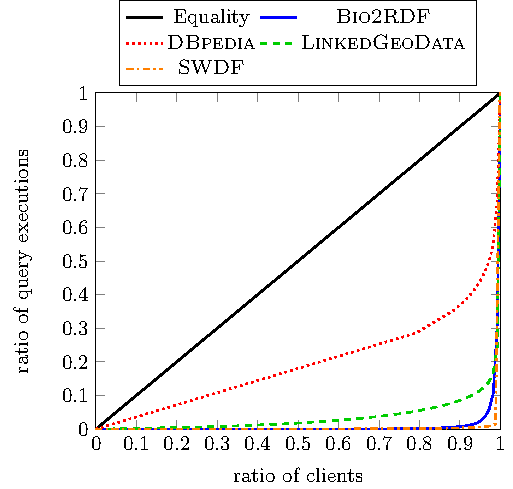
\includegraphics[width=\linewidth]{lorenz/client-lorenz-b2r}
\caption{Lorenz curve for distribution of executions per client}
\label{fig:client_lorenz}
\end{minipage}
\hfill
\begin{minipage}{0.49\textwidth}
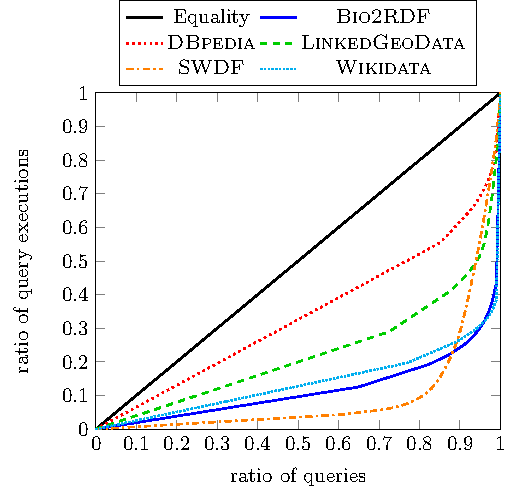
\includegraphics[width=\linewidth]{lorenz/query-lorenz-b2r}
\caption{Lorenz curve for distribution of executions per query}
\label{fig:query_lorenz}
\end{minipage}
\end{figure*}


\paragraph{Static and Runtime Statistics} Next, in order to characterise how complex the queries are to evaluate, in Table~\ref{tab:avgcomp} we present some relevant static and runtime statistics, where static statistics can be computed from the query string, while runtime statistics require evaluating the query locally (only queries that were successfully run are counted; see Table~\ref{tab:dsbstats} for statistics on runtime errors). Regarding runtimes, we recall that these were run with a one minute timeout, which represents the max runtime.
% TODO Complete statement below; it was just marked as blue and not as a todo note!
%{\color{blue}The minimum runtimes ...}
We see that \linkedgeodata contains the most costly queries to run, which appears to correlate with larger result sizes and a larger mean join-vertex degree. Relatively high runtimes are also seen for the \kegg dataset. The simplest queries to run are found in the \genage, \gendr and \taxonomy datasets. These results suggest, for example, that \linkedgeodata might be more suitable for consumers looking for a challenging benchmark.


\begin{table*}
\setlength{\tabcolsep}{1.4ex}
\centering
\caption{Comparison of the mean values of runtime statistics across all query logs (PVs = Project Variables, BGPs = Basic Graph Patterns, TPs = Triple Patterns, JVs = Join Vertices, MJVD = Mean Join Vertex Degree, MTPS = Mean Triple Pattern Selectivity)}
\label{tab:avgcomp}
\begin{tabular}{lrrrrrrrr} \toprule
\multirow{2}{*}{\textsc{Dataset}} & \multicolumn{5}{c}{\textsc{Static Statistics} (mean)} & \multicolumn{3}{c}{\textsc{Runtime Statistics}  (mean)} \\ 
 & PVs & BGPs & TPs & JVs & MJVD & MTPS & \textsc{Result Size} & \textsc{Runtime (sec)} \\ 
\cmidrule(r){1-1}\cmidrule(lr){2-6}\cmidrule(l){7-9}
\affymetrix & 1.93 & 1.06 & 1.10 & 0.03 & 0.06 & 0.82 & 12708.39 & 0.084\\
\biomodels & 1.24 & 1.04 & 1.42 & 0.37 & 0.75 & 0.57 & 4896.67 & 0.011\\
BIOPORTAL & 1.16 & 1.03 & 1.94 & 1.43 & 1.12 & 0.54 & 1699.48 & 0.004\\
\ctd & 2.56 & 1.05 & 1.08 & 0.02 & 0.04 & 0.85 & 24354.24 & 0.102\\
\dbpedia & 2.78 & 2.37 & 3.23 & 0.93 & 0.66 & 0.01 & 114038.38 & 0.164\\
\dbsnp & 1.09 & 1.02 & 1.04 & 0.02 & 0.04 & 0.97 & 757108.37 & 0.009\\
\drugbank & 2.61 & 1.05 & 1.93 & 0.69 & 0.91 & 0.66 & 119759.38 & 0.007\\
\genage & 1.88 & 1.00 & 1.09 & 0.04 & 0.13 & 0.99 & 1642.84 & 0.003\\
\gendr & 2.73 & 1.00 & 1.08 & 0.08 & 0.09 & 0.97 & 83.50 & 0.003\\
\go & 1.46 & 1.10 & 1.37 & 0.22 & 0.38 & 0.02 & 93806.20 & 0.046\\
\goa & 1.87 & 1.03 & 1.12 & 0.08 & 0.16 & 0.85 & 7692.26 & 0.016\\
\hgnc & 1.91 & 1.05 & 1.29 & 0.23 & 0.35 & 0.80 & 2419.43 & 0.019\\
\irefindex & 2.92 & 1.13 & 1.43 & 0.19 & 0.25 & 0.82 & 32200.76 & 0.077\\
\kegg & 2.27 & 1.15 & 1.31 & 0.13 & 0.18 & 0.33 & 175469.53 & 3.862\\
\linkedgeodata & 2.27 & 1.16 & 2.62 & 1.10 & 1.76 & 0.15 & 11055973.09 & 6.788\\
\linkedspl & 2.01 & 1.00 & 1.00 & 0.00 & 0.00 & 1.00 & 9503.41 & 0.014\\
\mgi & 2.04 & 1.04 & 1.11 & 0.05 & 0.06 & 0.84 & 2050.76 & 0.178\\
\ncbigene & 1.39 & 1.02 & 1.04 & 0.03 & 0.04 & 0.95 & 10731.33 & 0.021\\
\omim & 1.83 & 1.07 & 1.26 & 0.17 & 0.18 & 0.77 & 3505.54 & 0.020\\
\pharmgkb & 1.96 & 1.34 & 2.48 & 1.06 & 1.08 & 0.39 & 255.61 & 0.017\\
\sabiork & 2.96 & 1.05 & 1.06 & 0.01 & 0.02 & 0.88 & 1610.77 & 0.005\\
\sgd & 1.45 & 1.12 & 1.96 & 0.35 & 0.18 & 0.58 & 108951.60 & 0.058\\
\sider & 1.34 & 1.00 & 1.01 & 0.01 & 0.01 & 0.98 & 9703.86 & 0.010\\
\swdf & 4.04 & 3.37 & 3.97 & 0.45 & 0.92 & 0.03 & 37362.67 & 0.007\\
\taxonomy & 1.77 & 1.17 & 1.53 & 0.23 & 0.59 & 0.69 & 1928.75 & 0.004\\
\wikidata & 3.00 & 2.47 & 4.73 & 1.06 & 1.81 & 0.00 & 17817773.63 & 0.412\\
\wormbase & 1.56 & 1.25 & 2.05 & 0.65 & 0.87 & 0.98 & 9888.61 & 0.007\\
\midrule
Overall & 2.07 & 1.26 & 1.71 & 0.35 & 0.47 & 0.65 & 1126559.96 & 0.440\\
\bottomrule
\end{tabular}
\end{table*}

\paragraph{LSQ dataset statistics} The LSQ 2.0 dataset, describing 43.95 million executions of 11.56 million unique queries, contains 1.24~billion triples, split into 27 named graphs (one for each of the datasets listed).\footnote{We exclude some named graphs created by Virtuoso.}

\section{LSQ Adoption}
\label{sec:lsq_adoption}

In this section we present how LSQ has been adopted since its initial release with four logs in 2015. We organise this discussion following the motivational use cases we originally envisaged, as presented in Section~\ref{sec:usecase}.
Table~\ref{tab:logstats} provides an overview of the research works that have used LSQ, and the relevant use case(s) that they target. We now discuss these works in more detail; note that in the case of works that relate to multiple use cases, we will discuss them once in what we identify to be the ``primary'' related use case. We further discuss some works that have used the LSQ dataset for use cases beyond the six we had originally envisaged.

\begin{table*}
\centering
\setlength{\tabcolsep}{1.2ex}
\caption{Research works making use of the LSQ dataset since its initial release, ordered by year and then alphabetically by author name, with relevant use cases indicated (UC1: Custom Benchmarks; UC2: SPARQL Adoption; UC3: Caching; UC4: Usability; UC5: Optimisation; UC6: Meta-Querying)}
\label{tab:logstats}
\begin{tabular}{lcccccccc}
\hline
\textsc{Name} & \textsc{Year} & UC 1 & UC 2 & UC 3 & UC 4 & UC 5 & UC 6 & Other \\
\hline
Saleem et al.~\cite{SaleemMN15} & 2015 &	\checkmark  &  &  &  &   & &	\\
Arenas et al.~\cite{arenas2016reverse} & 2016 & \checkmark & & & \checkmark &  &  &  \\
Benedetti and Bergamaschi~\cite{benedetti2016model} & 2016 & & & & \checkmark &  & & \\
Georgala et al.~\cite{georgala2016efficient} & 2016 & &  &  &  &  & & \checkmark \\
Han et al.~\cite{han2016statistical} & 2016 & & \checkmark & & & \checkmark & & \\
Hernandez et al.~\cite{hernandez2016querying} & 2016 & \checkmark & & &  &  &   & \\
Knuth et al.~\cite{knuth2016scheduling} & 2016 & \checkmark &  & \checkmark &  &  &   & \\
Rico et al.~\cite{rico2016data} & 2016 & & & & & & \checkmark & \\
%Ngomo and Saleem \cite{ngomo2016federated} & 2016 & \checkmark & & &  &  & & \\
Schoenfisch and Stuckenschmidt~\cite{schoenfisch2016analyzing} & 2016 &  & \checkmark &  &  & \checkmark & & \\
Song et al.~\cite{song2016efficient} & 2016 & \checkmark &  &  &  & \checkmark & & \\


Bonifati et al.~\cite{BonifatiMT17} & 2017 & & \checkmark & & & \checkmark & & \\
Dellal et al.~\cite{dellal2017addressing} & 2017 &  & &  & \checkmark &  &  &  \\
Fokou et al.~\cite{FokouJHB17} & 2017 & & & & \checkmark & & \\
Stegemann and Ziegler~\cite{stegemann2017investigating} & 2017 &	\checkmark  & \checkmark &  & \checkmark & &  & \\
Thakkar et al.~\cite{thakkar2017trying} & 2017 & \checkmark &  &  &  &   &  &  \\

Akhtar et al.~\cite{akhtar2018change} & 2018 & \checkmark &  & \checkmark &  &  & & \\
Bonifati et al.~\cite{bonifati2018darql} & 2018 & & \checkmark &  &  & \checkmark & & \\
Darari et al.~\cite{darari2018completeness} & 2018 &  &  &  &  &   &  & \checkmark \\
Martens and Trautner~\cite{MartensT18} & 2018 & & & & & \checkmark & & \\
Salas and Hogan~\cite{SalasH18} & 2018 & \checkmark & & \checkmark  & & & & \\
Saleem et al.~\cite{saleem2018largerdfbench} & 2018 & \checkmark &  &  &  &   & &	\\
Saleem et al.~\cite{SaleemMSLN18} & 2018 & \checkmark &  &  &  &   & &	\\
Varga et al.~\cite{varga2018analytical} & 2018 & & & & & & \checkmark & \\
Viswanathan et al.~\cite{Viswanathan18} & 2018 & & & & \checkmark & & \\

Akhtar et al.~\cite{akhtar2019dynamic} & 2019 & \checkmark &  & \checkmark &  &  & & \\
Cheng and Hartig~\cite{cheng2019opt+} & 2019 & \checkmark & \checkmark &  &  & \checkmark & &	\\
Fafalios and Tzitzikas~\cite{fafalios2019many} & 2019 & &  &  &  &   & & \checkmark	 \\
Fernandez et al.~\cite{fernandez2019evaluating} & 2019 & \checkmark & & &  &  &   &  \\
Potoniec~\cite{Potoniec19} & 2019 & \checkmark & & & \checkmark & & & \\
Saleem et al.~\cite{SaleemSCBMN19} & 2019 & \checkmark &  &  &  &   & &	 \\
Thost and Dolby~\cite{thost2019qed} & 2019 & \checkmark &  &  &   &   & & \checkmark \\
Wang et al.~\cite{wang2019answering}  & 2019 & &  &  & \checkmark &  & & \\
Savafi et al.~\cite{safavi2019personalized}  & 2019 & & & \checkmark &  &  & & \\
Singh et al.~\cite{singh2019qaldgen}  & 2019 &\checkmark &  &  &  &  & & \checkmark \\
Azzam et al.~\cite{azzam2020smart}  & 2020 & \checkmark &  &  &  &  & & \\
Bigerl et al.~\cite{bigerl2020tentris}  & 2020 & \checkmark&  &  &  &  & & \\
Bonifati et al.~\cite{BonifatiMT20} & 2020 & & \checkmark & & \checkmark & \checkmark & & \\
Figueira et al.~\cite{FigueiraGKMNT20} & 2020 & & \checkmark & & &  \checkmark & & \\
Jian et al.~\cite{jian2020sparql}  & 2020 & \checkmark &  &  & \checkmark  &  & & \\
Zhang et al.~\cite{zhang2020revealing}  & 2020 & \checkmark & &  & \checkmark  &  & & \\

Aebeloe et al.~\cite{AebeloeMH21} & 2021 & \checkmark &  &  &  &  & & \checkmark \\
Almendros-Jimenez et al.~\cite{ALMENDROSJIMENEZ2021113772} & 2021 & \checkmark &   &  & \checkmark &  & & \\
Azzam et al.~\cite{AzzamAMKPH21}  & 2021 & \checkmark &  &  &  &  & & \\
Davoudian et al.~\cite{davoudian2021workload} & 2021 & \checkmark&   &  &  &  & & \\
Desouki et al.~\cite{9364498} & 2021 & \checkmark&   &  &  &  & & \\
Röder et al.~\cite{9364380}  & 2021 & \checkmark&   &  &  &  & & \\
Wang et al.~\cite{wang2021explaining} & 2021 & \checkmark&   &  & \checkmark &  & & \\
%Azzam et al.~\cite{AzzamAMKPH21}  & 2021 & \checkmark&   &  &  &  & & \\
\bottomrule
\end{tabular}
\end{table*}


\paragraph{UC1: Custom Benchmarks} LSQ has been adopted in various works for creating custom benchmarks. 

\begin{itemize}
\item Saleem et al.~\cite{SaleemMN15} present a framework for generating benchmarks that can be used to evaluate SPARQL endpoints under typical workloads; the benchmarks generate query types depending on the features of the queries submitted to the endpoint, where LSQ is used for testing. 
\item Later works by Saleem et al. further propose frameworks for generating benchmarks from LSQ for the purposes of evaluating query containment~\cite{SaleemMSLN18,saleem2017sqcframework} and federated query evaluation~\cite{saleem2018largerdfbench}, as well as comparing existing SPARQL benchmarks against LSQ in order to understand how representative they are of real workloads~\cite{SaleemSCBMN19}. 
\item Hern{\'a}ndez et al.~\cite{hernandez2016querying} present an empirical study of the efficiency of graph database engines for answering SPARQL queries over Wikidata; they refer to LSQ to verify that the query shapes considered for evaluation correspond with other analyses of real-world SPARQL queries. 
\item Fern{\'a}ndez et al.~\cite{fernandez2019evaluating} evaluate various archiving techniques and querying strategies for RDF archives that store historical data; in their evaluation, they select the 200 most frequent triple patterns from the \dbpedia query set in LSQ. 
\item Azzam et al.~\cite{azzam2020smart} use LSQ for retrieving highly-demanding queries from the dataset in order to evaluate their system for dividing the load processed by different SPARQL servers. 
\item Bigerl et al.~\cite{bigerl2020tentris} develop a tensor-based triple store, where they used LSQ as input to the FEASIBLE framework to generate a custom benchmark. 
\item Azzam et al.~\cite{AzzamAMKPH21} present a system that dynamically delegates query processing load between clients and servers. The authors use the Linked Data Fragments client/server approach improving it with the aforementioned technique and use 16 queries from LSQ to complement their evaluation.
\item Davoudian et al.~\cite{davoudian2021workload} present a system that partitions graphs depending on the access frequency to their nodes. In this way the system implements workload-aware partitioning. The authors use LSQ for evaluating their approach.
\item Desouki et al.~\cite{9364498} propose a method to generate synthetic benchmark data. To generate these synthetic data they use other RDF graphs available, such as \swdf and \dbpedia 2016. They benchmark their approach using queries from LSQ.
\item R\"oder et al.~\cite{9364380} develop a method to predict the performance of knowledge graph query engines; to do so the authors use a stochastic generation model that is able to generate graphs of arbitrary sizes similar to the input graph. They use LSQ as a benchmark of real-world queries.
\end{itemize}

%Saleem et al.~\cite{SaleemMN15,SaleemMSLN18} create a framework, called SQC-Framework, for generating benchmarks to evaluate \textit{query containment}---i.e., deciding if the result set of a given query is included in that of another given query---using the LSQ meta-data and clustering methods to select diverse real-world queries.

%Saleem et al.~\cite{SaleemMSLN18} create a framework, called SQC-Framework, for generating benchmarks to evaluate \textit{query containment}---i.e., deciding if the result set of a given query is included in that of another given query---using the LSQ meta-data and clustering methods to select diverse real-world queries.

%Saleem et al.~\cite{saleem2018largerdfbench} present a benchmark for federated SPARQL queries that span several distributed RDF datasets; to generate these queries the authors use LSQ.

%Ngonga Ngomo and Saleem~\cite{ngomo2016federated} present the challenges and opportunities in federated query processing, showing the need of using real SPARQL queries in the evaluation benchmarks, highlighting the use of LSQ to know which are the most popular queries a system should process most frequently. Aidan: I think this is covered by feasible.

% custom benchmark

%Saleem et al.~\cite{SaleemSCBMN19} provide an analysis of how to chose the most suitable benchmark for evaluating triple stores in practical settings, providing a a comparative analysis of existing SPARQL benchmarks with LSQ.

% custom benchmark


\paragraph{UC2: SPARQL Adoption}
\label{sec-sparql_adoption_uc}

Other works have used LSQ to understand how SPARQL is being used in practice. 


\begin{itemize}
\item Han et al.~\cite{han2016statistical} provide a statistical analysis of the queries of LSQ, surveying both syntactic features, such as the number of triple patterns, the SPARQL features used, the frequency of well-designed patterns; as well as semantic properties, such as montonicity, weak-monotonicity, non-monotonicity and satisfiability.
\item Bonifati et al.~\cite{BonifatiMT17,bonifati2018darql} conduct detailed analysis of the queries in various logs, including LSQ; they study a variety of phenomena in these queries, including their shape, their (hyper)treewidth, common abstract patterns found in the property paths, ``streaks'' that represent a sequence of user reformulations from a seed query, and more besides.
\end{itemize}   

\paragraph{UC3: Caching}
\label{sec-caching_uc}

LSQ can also be used to simulate real workloads for systems that explore caching techniques. 

\begin{itemize}
\item Knuth et al.~\cite{knuth2016scheduling} propose a middleware component to which applications register and get notifications when the results of their SPARQL queries change; the authors study the problem of scheduling refresh queries for a large number of registered queries and use LSQ to validate their approach. 
\item Akhtar et al.~\cite{akhtar2018change,akhtar2019dynamic} propose an approach to capture changes in an RDF dataset and update a cache system in front of the SPARQL endpoint exposing that data; their approach consists of a change metric that quantifies the changes in an RDF dataset, and a weighting function that assigns importance to recent changes; they use LSQ to verify their approach for real workloads. 
\item Salas and Hogan~\cite{SalasH18} propose a method for query canonicalisation, which consists in mapping congruous queries---i.e., queries that are equivalent modulo variable names---to the same query string; their main use case is to increase the hit rate of SPARQL caches, where they use LSQ to test efficiency on real-world queries and to see how many congruent queries can be found in real workloads.
\item Savafi et al.~\cite{safavi2019personalized} study SPARQL adoption using LSQ so they can later provide queries to summarise the Knowledge Graphs such that they can be more efficiently accessed from and stored on mobile devices with limited resources.
\end{itemize}

\paragraph{UC4: Usability}
\label{sec-usability_uc}

LSQ also has applications for improving the usability of SPARQL endpoints. 

\begin{itemize}
\item Arenas et al.~\cite{arenas2016reverse} propose a method for reverse-engineering SPARQL queries, which attempts to construct a query that will return a given set of positive examples as results, but not a second set of negative examples; the authors use LSQ to show that the approach scales well in the data size, number of examples, and in the size of the smallest query that fits the data. 
\item Benedetti and Bergamaschi~\cite{benedetti2016model} present a system (LODeX) that allows users to explore SPARQL endpoints more easily through a formal model defined over the endpoint schema; they show that LODeX is able to generate 77.6\% of the 5 million queries contained in the original LSQ dataset. 
\item Dellal et al.~\cite{dellal2017addressing} proposes query relaxation methods for queries with empty results, based on finding minimal failing subqueries (generating empty results) and maximal succeeding subqueries (generating non-empty results) to aid the user~\cite{FokouJHB17}. The paper refers to LSQ to establish that queries with empty results are common in practice.
\item Stegemann and Ziegler~\cite{stegemann2017investigating} propose new operators for the SPARQL language that allow for composing path queries more easily; the authors evaluated their approach with a user study and analysis of the extent to which their language is able to express the real-world queries found in LSQ.
\item Viswanathan et al.~\cite{Viswanathan18} propose a different form of query relaxation, which generalises a specific resource to a variable on which specific restrictions are added that correspond to relevant characteristics of the resource; they use LSQ to understand how entities are queried in practice. 
\item Potoniec~\cite{Potoniec19} proposes an interactive system for learning SPARQL queries from positive and negative examples;\footnote{Notably the system is called Learning SPARQL Queries (LSQ).} he uses the \dbpedia queries of LSQ for experiments. 
\item Wang et al.~\cite{wang2019answering} present an approach for explaining missing results for a SPARQL query---based on answering ``\textit{why-not}'' questions that ask why a specific result is not included---to help users refine their initial queries; the authors search LSQ for queries useful for their approach. 
\item Bonifati et al.~\cite{BonifatiMT20} analyse ``streaks'' in DBpedia query logs,\footnote{In fact, these logs were gathered directly from OpenLink, though we include discussion since similar analysis could have been applied to the LSQ logs, and LSQ logs where used in other analyses.} where a streak is defined as a sequence of similar queries in chronological order, capturing the idea of a user refining and/or extending an initial query towards a final query.
\item Jian et al.~\cite{jian2020sparql} use LSQ to evaluate their approach for SPARQL query relaxation (to generalise users' queries) and query restriction (to refine users' queries) based on approximation and heuristics.
\item Zhang et al.~\cite{zhang2020revealing} propose a method to model client behaviour when formulating SPARQL queries in order to predict their intent and optimise queries. They use LSQ for their evaluation.
\item Almendros-Jimenez et al.~\cite{ALMENDROSJIMENEZ2021113772} present two methods for discovering and diagnosing ``wrong'' SPARQL queries based on ontology reasoning. They evaluate their approach using LSQ queries.
\item Wang et al.~\cite{wang2021explaining} focus on providing explanations for SPARQL query similarity measures. The authors provide similarity scores using several explainable models based on Linear Regression, Support Vector Regression, Ridge Regression, and Random Forest Regression. They use LSQ to evaluate their query classification.
\end{itemize}

\paragraph{UC5: Optimisation}
\label{sec-optimisation_uc}

The LSQ dataset can also be used to identify and study fragments that are commonly used in practice and can be evaluated efficiently using dedicated algorithms. 
\begin{itemize}
\item The aforementioned analyses by Han et al.~\cite{han2016statistical} and Bonifati et al.~\cite{BonifatiMT17,bonifati2018darql} suggest that well-designed patterns, queries of bounded treewidth, etc., make for promising fragments. 
\item In the context of probabilistic Ontology-Based Data Access (OBDA), Schoenfisch and Stuckenschmidt~\cite{schoenfisch2016analyzing} analyse the ratio of safe queries---whose evaluation is tractable in data complexity---versus unsafe queries---whose evaluation is $\#$P-hard; they show that over 97.9\% of the LSQ queries are safe, and can be efficiently evaluated.
\item Song et al.~\cite{song2016efficient} use LSQ to analyse how nested \texttt{OPTIONAL} clauses affect query response times; they propose a way to approximate solutions for deeply-nested well-designed patterns.
\item Martens and Trautner~\cite{MartensT18} later take the property paths extracted by Bonifati et al.~\cite{BonifatiMT17} from LSQ and other sources, defining \textit{simple transitive expressions} that subsume almost all property path expressions seen in practice, while allowing more efficient evaluation than the general case. 
\item Cheng and Hartig~\cite{cheng2019opt+} introduce a monotonic version of the \texttt{OPTIONAL} operator to SPARQL called \texttt{OPT+}; a possible downside of the operator is an increase in query result sizes, where they use the LSQ dataset to study how \texttt{OPTIONAL} and \texttt{OPT+} behave for real-world queries.
\item Building upon the work of Martens and Trautner~\cite{MartensT18}, Figueira et al.~\cite{FigueiraGKMNT20} specifically study the containment problem for restricted classes of Conjunctive Regular Path Queries (CRPQs), which are akin to BGPs with property paths; aside from complexity results, they show the coverage of the different classes for logs that include LSQ~\cite{BonifatiMT20}.
\end{itemize}

%In~\cite{khouri2018lod} is just a reference in the state of the art.


\paragraph{UC6: Meta-Querying}
\label{sec-metaquerying_uc}

A handful of works have also used LSQ in the context of meta-querying, where queries are found based on the resources they contain. 

\begin{itemize}
\item Rico et al.~\cite{rico2016data} observe that analogous \dbpedia properties are often defined in two distinct namespaces---e.g., \texttt{dbo:birthPlace} and \texttt{dbp:birthPlace}---where they propose methods to automatically expand SPARQL queries to capture solutions involving analogous properties; they show that only 0.2\% of the \dbpedia queries in LSQ mention properties from both namespaces.
\item Varga et al.~\cite{varga2018analytical} provide an RDF-based metamodel for BI 2.0 systems, which allows for capturing the schema of a dataset, as well as previous queries that have been posed against that dataset by other users; the authors propose to re-use parts of the LSQ vocabulary in their model; they further instantiate their model using LSQ to retrieve queries asked about countries.
\end{itemize} 

\paragraph{Other use cases} A number of works have used LSQ (mostly for evaluation) in contexts that were not originally anticipated by the aforementioned use cases.

\begin{itemize}
\item Georgala et al.~\cite{georgala2016efficient} propose a method to predict temporal relations between events represented by RDF resources following Allen's interval algebra; they use LSQ to validate their approach considering query executions as events.  
\item Darari et al.~\cite{darari2018completeness} present a theoretical framework for augmenting RDF data sources with completeness statements, which allows for reasoning about the completeness of SPARQL query results; they evaluate their method using LSQ.
\item Fafalios and Tzitzikas~\cite{fafalios2019many} present a query evaluation strategy, called SPARQL-LD, that combines link traversal and query processing at SPARQL endpoints; they provide a method for checking if a SPARQL query can be answered through link traversal, and analyse a large corpus of real SPARQL query logs---including LSQ---for finding the frequency and distribution of answerable and non-answerable query patterns; they also use LSQ to evaluate their approach.
\item Singh et al.~\cite{singh2019qaldgen} use the LSQ vocabulary for providing a benchmark for Question Answering over Linked Data. The authors use the LSQ vocabulary to represent the SPARQL query related features prior to generating the benchmark. 
\item Thost and Dolby~\cite{thost2019qed} present QED: a system for generating concise RDF graphs that are sufficient to produce solutions from a given query, which can be used for benchmarking, for compliance testing, for training query-by-example models, etc.; they apply their system over LSQ queries to generate datasets from \dbpedia. 
\item Aebeloe et al.~\cite{AebeloeMH21} present a decentralised architecture based on blockchain that allows users to propose updates to faulty or outdated data, tracing back their origin, and query older versions of the data. They use LSQ queries for their evaluation. 
\end{itemize}

\paragraph{Discussion} Per Table~\ref{tab:logstats}, we see that the original version of LSQ has been used in a wide variety of research works for a variety of purposes. Complementing other SPARQL query logs such as Wikidata's~\cite{MalyshevKGGB18}, we believe that LSQ~2.0, with its extended set of queries, will likewise serve as a useful resource to help align the theory and practice of SPARQL research.

\section{Conclusions and Future Directions}
\label{sec:conclusion}

In this paper, we have described the Linked SPARQL Queries v.2 (LSQ~2.0) dataset, which represents queries in logs as RDF, allowing clients to quickly find real-world queries that may be of interest to them. We have described a number of use cases for LSQ, including the generation of custom benchmarks, the analysis of how SPARQL is used in practice, the evaluation of caching systems, the exploration of techniques to improve the usability of SPARQL services, the targeted optimisation of queries with characteristics commonly found in real workloads, as well as the ability to find queries relating to specific resources. We then described the model and vocabulary used to represent LSQ, including static features of queries, a SPIN representation, provenance encoding the agents and endpoints from which the query originate, as well as runtime statistics generated through local executions of the queries against their corresponding dataset. We then discussed how LSQ is published, thereafter describing the datasets and queries featured in the current version of LSQ. Finally we discussed how LSQ has been used for research purposes since its initial release in 2015.

As discussed in Section~\ref{sec:lsq_adoption}, since its initial release, LSQ has been adopted by a variety of research works for a variety of purposes. In terms of future directions, we will look to continue adding further logs with further queries to the dataset. Looking at how LSQ has been adopted in the literature has also revealed ways in which the metadata for LSQ could be extended in a future version, such as to add information about monotonicity and satisfiability~\cite{han2016statistical}, or information about (hyper)treewidth~\cite{BonifatiMT17,bonifati2018darql}, for example. It may also be useful to provide a canonical version of the query string~\cite{SalasH18}; this could perhaps be leveraged, for example, when evaluating caching methods. Another useful feature would be to add questions in natural language that verbalise each query, which could be used, for example, in order to create datasets for training and testing question answering systems, as well as enabling users to find relevant queries through keyword search; given the large number of queries in the dataset, an automated approach may be applicable~\cite{NgomoBULG13}.

As discussed by Martens and Trautner~\cite{MartensT19}, query logs allow to bridge the theory and practice of SPARQL. They serve an important role, ensuring that the research conducted by the community is guided by the requirements and trends that emerge in practice. We thus believe that LSQ~(2.0) will continue to serve an important role in SPARQL research in the coming years.


